% Options for packages loaded elsewhere
\PassOptionsToPackage{unicode}{hyperref}
\PassOptionsToPackage{hyphens}{url}
%
\documentclass[
  english,
  man]{apa6}
\author{\phantom{0}}
\date{}

\usepackage{amsmath,amssymb}
\usepackage{lmodern}
\usepackage{iftex}
\ifPDFTeX
  \usepackage[T1]{fontenc}
  \usepackage[utf8]{inputenc}
  \usepackage{textcomp} % provide euro and other symbols
\else % if luatex or xetex
  \usepackage{unicode-math}
  \defaultfontfeatures{Scale=MatchLowercase}
  \defaultfontfeatures[\rmfamily]{Ligatures=TeX,Scale=1}
\fi
% Use upquote if available, for straight quotes in verbatim environments
\IfFileExists{upquote.sty}{\usepackage{upquote}}{}
\IfFileExists{microtype.sty}{% use microtype if available
  \usepackage[]{microtype}
  \UseMicrotypeSet[protrusion]{basicmath} % disable protrusion for tt fonts
}{}
\makeatletter
\@ifundefined{KOMAClassName}{% if non-KOMA class
  \IfFileExists{parskip.sty}{%
    \usepackage{parskip}
  }{% else
    \setlength{\parindent}{0pt}
    \setlength{\parskip}{6pt plus 2pt minus 1pt}}
}{% if KOMA class
  \KOMAoptions{parskip=half}}
\makeatother
\usepackage{xcolor}
\IfFileExists{xurl.sty}{\usepackage{xurl}}{} % add URL line breaks if available
\IfFileExists{bookmark.sty}{\usepackage{bookmark}}{\usepackage{hyperref}}
\hypersetup{
  pdflang={en-EN},
  hidelinks,
  pdfcreator={LaTeX via pandoc}}
\urlstyle{same} % disable monospaced font for URLs
\usepackage{graphicx}
\makeatletter
\def\maxwidth{\ifdim\Gin@nat@width>\linewidth\linewidth\else\Gin@nat@width\fi}
\def\maxheight{\ifdim\Gin@nat@height>\textheight\textheight\else\Gin@nat@height\fi}
\makeatother
% Scale images if necessary, so that they will not overflow the page
% margins by default, and it is still possible to overwrite the defaults
% using explicit options in \includegraphics[width, height, ...]{}
\setkeys{Gin}{width=\maxwidth,height=\maxheight,keepaspectratio}
% Set default figure placement to htbp
\makeatletter
\def\fps@figure{htbp}
\makeatother
\setlength{\emergencystretch}{3em} % prevent overfull lines
\providecommand{\tightlist}{%
  \setlength{\itemsep}{0pt}\setlength{\parskip}{0pt}}
\setcounter{secnumdepth}{-\maxdimen} % remove section numbering
% Make \paragraph and \subparagraph free-standing
\ifx\paragraph\undefined\else
  \let\oldparagraph\paragraph
  \renewcommand{\paragraph}[1]{\oldparagraph{#1}\mbox{}}
\fi
\ifx\subparagraph\undefined\else
  \let\oldsubparagraph\subparagraph
  \renewcommand{\subparagraph}[1]{\oldsubparagraph{#1}\mbox{}}
\fi
% Manuscript styling
\usepackage{upgreek}
\captionsetup{font=singlespacing,justification=justified}

% Table formatting
\usepackage{longtable}
\usepackage{lscape}
% \usepackage[counterclockwise]{rotating}   % Landscape page setup for large tables
\usepackage{multirow}		% Table styling
\usepackage{tabularx}		% Control Column width
\usepackage[flushleft]{threeparttable}	% Allows for three part tables with a specified notes section
\usepackage{threeparttablex}            % Lets threeparttable work with longtable

% Create new environments so endfloat can handle them
% \newenvironment{ltable}
%   {\begin{landscape}\centering\begin{threeparttable}}
%   {\end{threeparttable}\end{landscape}}
\newenvironment{lltable}{\begin{landscape}\centering\begin{ThreePartTable}}{\end{ThreePartTable}\end{landscape}}

% Enables adjusting longtable caption width to table width
% Solution found at http://golatex.de/longtable-mit-caption-so-breit-wie-die-tabelle-t15767.html
\makeatletter
\newcommand\LastLTentrywidth{1em}
\newlength\longtablewidth
\setlength{\longtablewidth}{1in}
\newcommand{\getlongtablewidth}{\begingroup \ifcsname LT@\roman{LT@tables}\endcsname \global\longtablewidth=0pt \renewcommand{\LT@entry}[2]{\global\advance\longtablewidth by ##2\relax\gdef\LastLTentrywidth{##2}}\@nameuse{LT@\roman{LT@tables}} \fi \endgroup}

% \setlength{\parindent}{0.5in}
% \setlength{\parskip}{0pt plus 0pt minus 0pt}

% \usepackage{etoolbox}
\makeatletter
\patchcmd{\HyOrg@maketitle}
  {\section{\normalfont\normalsize\abstractname}}
  {\section*{\normalfont\normalsize\abstractname}}
  {}{\typeout{Failed to patch abstract.}}
\patchcmd{\HyOrg@maketitle}
  {\section{\protect\normalfont{\@title}}}
  {\section*{\protect\normalfont{\@title}}}
  {}{\typeout{Failed to patch title.}}
\makeatother
\shorttitle{SHORTTITLE}
\usepackage{csquotes}
\usepackage{float}
\usepackage{sectsty}
\usepackage{lscape}
\newcommand{\blandscape}{\begin{landscape}}
\newcommand{\elandscape}{\end{landscape}}
\ifXeTeX
  % Load polyglossia as late as possible: uses bidi with RTL langages (e.g. Hebrew, Arabic)
  \usepackage{polyglossia}
  \setmainlanguage[]{english}
\else
  \usepackage[main=english]{babel}
% get rid of language-specific shorthands (see #6817):
\let\LanguageShortHands\languageshorthands
\def\languageshorthands#1{}
\fi
\ifLuaTeX
  \usepackage{selnolig}  % disable illegal ligatures
\fi


\affiliation{\phantom{0}}

\begin{document}

\hypertarget{chapitre-5-les-tests-duxe9quivalence}{%
\section{Chapitre 5 : Les tests d'équivalence}\label{chapitre-5-les-tests-duxe9quivalence}}

Lorsqu'on applique un test d'hypothèse, l'hypothèse nulle la plus couramment définie est celle d'absence d'effet ou de différence entre les groupes (\textbf{nickerson\_null\_2000?}). Il arrive également parfois que les chercheurs définissent un intervalle de valeur comme hypothèse nulle, mais le plus souvent, cet intervalle est borné par la valeur 0 (\textbf{nickerson\_null\_2000?}), on parle alors d'hypothèse unilatérale. Avec cette stratégie, le rejet de l'hypothèse nulle constitue un soutien en faveur de la présence d'un effet non nul, par contre, le non-rejet de l'hypothèse nulle ne peut être interprété comme un soutien en faveur de l'absence d'effet. Pourtant, il arrive souvent que des chercheurs l'interprètent de la sorte (\textbf{anderson\_theres\_2016?}). (\textbf{finch\_reporting\_2001?}), par exemple, ont rapporté que parmi 150 articles publiés entre 1940 et 1999 dans le \emph{JAP} (\emph{Journal of Applied Psychology}), 38\% interprétaient un résultat non significatif comme une acceptation de l'hypothèse nulle. Plus récemment, (\textbf{lakens\_equivalence\_2017?}) a noté que l'expression ``pas d'effet'' a été utilisée dans 108 articles publiés dans \emph{Social Psychological and Personality Science} avant août 2016 et que dans presque tous les cas, c'était sur base du non-rejet de l'hypothèse nulle que cette conclusion était tirée. Cette erreur d'interprétation est également fréquemment commise dans le cadre des études de réplication. Anderson et Maxwell (2016), par exemple, ont analysé 50 réplications d'études publiées en 2013 dans PsycINFO. Ils ont noté que 14 études affirmaient avoir obtenu des effets ``nuls'' (interprété comme un échec à la réplication), et tous l'ont fait sur base de l'acceptation d'une hypothèse nulle d'absence d'effet. C'est par exemple de cette manière qu'on été réalisées la plupart des tentatives de réplications de la célèbre étude de Bem (\textbf{anderson\_theres\_2016?}).

A travers ce chapitre, notre premier objectif sera d'expliquer pourquoi interpréter le non-rejet de l'hypothèse d'absence d'effet comme un soutien en faveur d'une absence d'effet n'est pas une bonne stratégie. Nous introduirons ensuite les tests d'équivalence qui permettent d'obtenir un soutien en faveur d'un effet jugé non pertinent, et plus particulièrement le TOST (Two One-sided test). Nous verrons que l'aspect le plus compliqué de la réalisation du TOST est la définition des bornes d'équivalence. Pour cette raison, notre troisième objectif sera de fournir quelques pistes en vue de définir ces bornes. Pour finir, nous présenterons un article dans lequel nous comparons le TOST à la SGPV (Second Generation \emph{P}-Value), une stratégie récemment développée par Blume et al.~(2018).

\hypertarget{limites-de-lapproche-traditionnelle}{%
\subsection{Limites de l'approche traditionnelle}\label{limites-de-lapproche-traditionnelle}}

Lorsqu'on teste une hypothèse nulle, il y a deux conclusions possibles : soit ont la rejette, soit on ne la rejette pas. Si rejeter l'hypothèse nulle amène à conclure en faveur de l'hypothèse alternative, ne pas la rejeter ne permet pas de conclure en faveur de l'hypothèse nulle. Au mieux, cela nous montre que les données ne sont pas incompatibles avec l'hypothèse nulle, mais cela ne veut en aucun cas dire qu'elles ne sont compatibles avec aucune autre hypothèse. Afin de l'illustrer, la Table 1 résume les résultats de simulations Monte Carlo pour un ensemble de 42 scénarios qui varient en fonction de la taille des échantillons (\(n_j\)) et de la différence entre les moyennes de population dont sont extraits les échantillons (\(\mu_1-\mu_2\)). Pour chaque scénario, à 100,000 reprises, nous avons généré aléatoirement une paire d'échantillons indépendants, réalisé un test \(t\) de Student pour échantillons indépendants et extrait la \(p\)-valeur du test.\footnote{Rappelons que le test de Student repose sur la condition peu réaliste d'homogénéité des variances de population. Nous avons assuré le respect de cette condition en générant systématiquement deux échantillons extraits de populations aux variances identiques. Dans la mesure où le message-clé de cette illustration ne dépend pas du test utilisé, nous avons fait ce choix par facilité, en vue de simplifier l'équation de l'erreur standard de la différence de moyennes, qui sera ultérieurement mentionnée.} Ensuite, nous avons calculé la proportion d'itérations associées à une \(p\)-valeur supérieure à .05, nous amenant à ne pas rejeter l'hypothèse nulle lorsqu'on travaille avec un risque alpha de 5\% (ce risque alpha étant communément accepté par la majorité des chercheurs; Meyners, 2012). Lorsque l'hypothèse nulle est fausse (toutes les colonnes de la Table 1, à l'exception de la première), cette proportion correspond au taux d'erreur de type II (communément appelé \(\beta\)).

\begin{flushleft}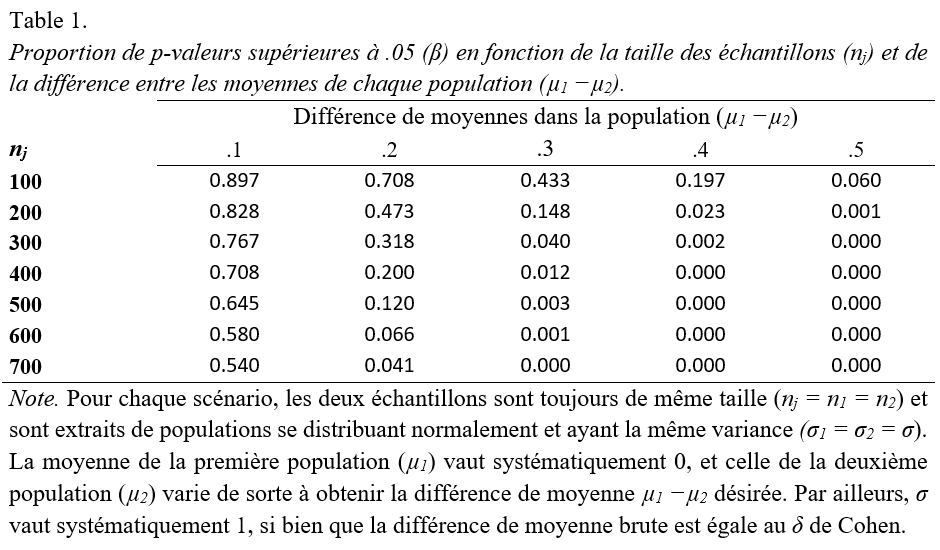
\includegraphics[width=0.95\linewidth]{C:/Users/mdelacre/Documents/Github project/thesis/Chapitre 5/Illustration/Table1} \end{flushleft}
\newpage

Pour éviter d'interpréter un test peu puissant comme un soutien en faveur de l'hypothèse nulle, l'approche de la puissance est devenue l'approche par défaut dans les années 80 pour tester l'équivalence (\textbf{meyners\_equivalence\_2012?}). A travers cette approche qui est restée très populaire (\textbf{quertemont\_how\_2011?}), dans un premier temps, on définit ce que l'on considère comme étant la plus petite valeur d'intérêt (en anglais, le ``SESOI'' pour ``Smaller Effect Size of Interest''), c'est-à-dire la taille d'effet minimale requise pour considérer qu'un effet est pertinent. Ensuite, on estime la puissance de notre test à détecter un effet de cette taille\footnote{On parle d'estimation et non de mesure, car la puissance du test dépend de $\sigma$, l'écart-type de la population, qu'on ne connaît pas et devra donc estimer sur base de $S$, l'écart-type de l'échantillon (Schuirmann,1987).} et si cette estimation atteint une valeur jugée satisfaisante (en général, 80\%), alors on considère que l'on peut interpréter le non-rejet de l'hypothèse nulle d'absence d'effet comme soutien en faveur de l'équivalence (\textbf{quertemont\_how\_2011?}; \textbf{meyners\_equivalence\_2012?}; \textbf{schuirmann\_comparison\_1987?}). L'idée sous-jacente est que si l'effet est au moins aussi grand que les bornes de la zone d'équivalence, sur le long terme, on devrait le plus souvent rejeter l'hypothèse nulle. Par conséquent, un non-rejet de l'hypothèse nulle devrait généralement signifier que l'effet n'atteint pas le SESOI et donc, que l'effet observé n'est pas pertinent. Bien que ce raisonnement puisse sembler tentant, de prime abord, il présente d'importantes limites.

Premièrement, le test n'a pas de bonnes propriétés asymptotiques. Ceci est illustré au sein de la Table 2, dans laquelle nous envisageons les mêmes scénarios que dans la Table 1 et ajoutons une contrainte de puissance : nous décidons qu'on ne peut conclure à l'équivalence que si l'on atteint une puissance de 80\% pour détecter une différence de moyenne de .3. On constate qu'avec 100 sujets par groupes, aucune itération n'amènera à conclure à l'équivalence, pas même lorsque la différence entre les moyennes de population vaut 0. Cela s'explique par le fait que l'on n'atteint jamais la puissance minimale de \(80\%\).\footnote{Avec 100 sujets par groupe, on estime la puissance du test à $80\%$ lorsque l'estimation $d$ de Cohen vaut .3981. Par conséquent, un test sera susceptible de conclure à l'équivalence si les bornes de la zone d'équivalence, exprimée en mesure standardisée $d$ de Cohen, sont supérieures ou égales à .3981. Lorsqu'on fixe les bornes aux différences de moyennes $\pm .3$, cela n'est possible que si $S$ est inférieur ou égal à .7535. En effet, $d=\frac{\theta}{S} \leftrightarrow .3981 = \frac{.3}{S} \leftrightarrow S = \frac{.3}{.3981}=.7535$.  Or, avec 100 sujets par groupe, aucune estimation $S$ ne sera inférieure ou égale à .7535 lorsque $\sigma$ vaut 1.} Par contre, une fois les échantillons assez grands pour s'assurer une puissance de \(80\%\) pour détecter une différence entre les moyennes de population de .3, lorsque la différence entre les moyennes de population est non nulle, la proportion d'itérations qui amènent à conclure à l'équivalence diminue à mesure que la taille des échantillons augmente. Par exemple, lorsque la différence de moyennes vaut .1 au niveau des populations, on conclura à l'équivalence dans \(81\%\) des itérations avec 200 sujets par groupe, contre seulement \(54\%\) des itérations avec 700 sujets par groupe.\footnote{En comparant les Tables 1 et 2, on constate qu'avec 200 sujets par groupes, les proportions d'itérations de chaque scénario qui amènent à conclure à l'équivalence, dans la Table 2, sont inférieures aux proportions d'itérations de chaque scénario qui amènent à ne pas rejeter l'hypothèse nulle, dans la Table 1. Plus les échantillons sont grands, moins on observera d'écart entre les 2 tables car la proportion d'itérations qui ne pourront amener à conclure à l'équivalence en raison d'un manque de puissance diminuera. En effet, plus la taille des échantillons sera grande, plus la valeur maximale de $S$ permettant d'assurer la puissance des $80\%$ sera élevée. Par exemple, avec 200 sujets par groupes, la valeur maximale autorisée pour $S$ sera de $\frac{.3}{.2808}=1.07$. Avec 300 sujets par groupes, la valeur maximale autorisée pour $S$ sera de $\frac{.3}{.2291}=1.31$. Par conséquent, plus les tailles d'échantillons seront grandes, moins il sera probable que $S$ dépasse le seuil autorisé.}

\begin{flushleft}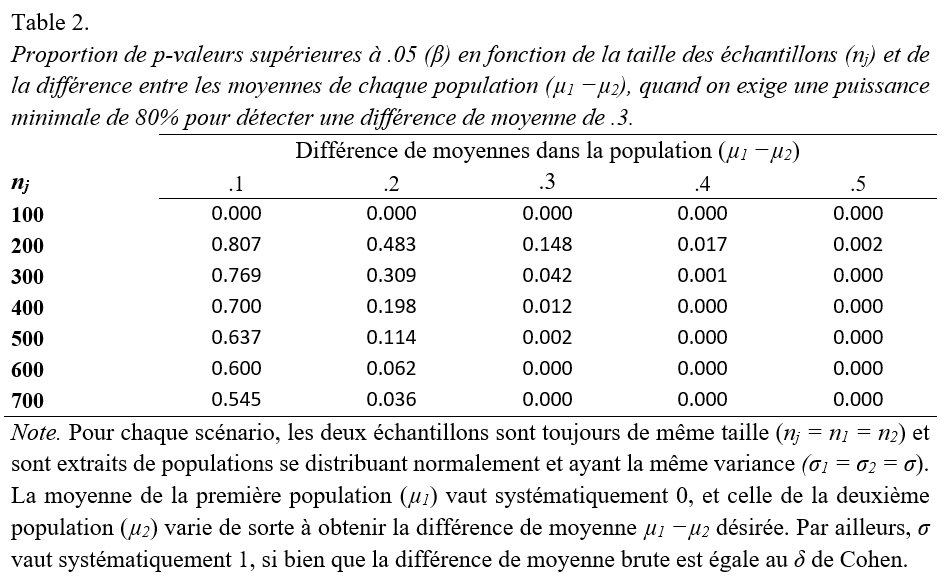
\includegraphics[width=0.95\linewidth]{C:/Users/mdelacre/Documents/Github project/thesis/Chapitre 5/Illustration/Table2} \end{flushleft}

Deuxièmement, pour une taille d'échantillon donnée, plus l'erreur (la variabilité des scores au sein de chaque groupe) sera grande (\textbf{meyners\_equivalence\_2012?}; \textbf{schuirmann\_comparison\_1987?}), plus la probabilité de conclure à l'équivalence augmentera. Ce dernier point est illustré au sein de la Figure \ref{fig:schuirman2}, dans le contexte de la comparaison de deux moyennes. Sur l'axe des abscisses, on représente différentes estimations de la différence de moyenne (\(\bar{X_1}-\bar{X_2}\)) et sur l'axe des ordonnées, la précision des estimations \(\bar{X_1}-\bar{X_2}\) (\(S\sqrt{\frac{2}{n}}\) correspond à l'estimation de l'erreur standard de \(\bar{X_1}-\bar{X_2}\), avec \(S\) étant l'écart-type poolé et \(n\) la taille de chaque échantillon, lorsque les échantillons ont tous les deux la même taille et sont extraits de population ayant la même variance).\footnote{Par facilité, à l'instar de Schuirman (1987), on envisage le cas où les échantillons sont de même taille et que l'on suppose que la condition d'homogénéité des variances est respectée. Notons cependant que d'après Schuirman, ce raisonnement peut être généralisé aux scénarios où les deux échantillons n'ont pas la même taille et sont extraits de population n'ayant pas la même variance.} Le triangle grisé représente l'ensemble des combinaisons estimation/précision qui vont amener à conclure à l'équivalence, avec l'approche de la puissance, lorsqu'on travaille avec des échantillons de taille 50, en acceptant un risque \(\alpha\) de 5\% et en exigeant une puissance minimale de 80\% pour détecter une différence de 20 unités (\(|\theta_j=20|,\;j=1,2\)). Dans cet exemple, pour toutes les valeurs de \(S\sqrt{\frac{2}{n}}\) supérieures à 7.07, aucune estimation de différence de moyennes ne permettra de conclure à l'équivalence (pas même 0) puisque la puissance du test à détecter une différence de 20 unités est inférieure à 80\%. Pour toutes les valeurs de \(S\sqrt{\frac{2}{n}}\) inférieures à 7.07, on constate que plus notre estimation de \(\bar{X_1}-\bar{X_2}\) est précise (lorsqu'on se déplace du haut vers le bas, sur l'axe des ordonnées), plus l'estimation doit être proche de 0 pour pouvoir conclure à l'équivalence. Comme on peut le voir à travers le triangle hachuré sur la Figure 10, cette propriété peu désirable n'est pas partagée par le TOST, un test d'équivalence que nous allons décrire ci-après (\textbf{schuirmann\_comparison\_1987?}).

\begin{figure}

{\centering 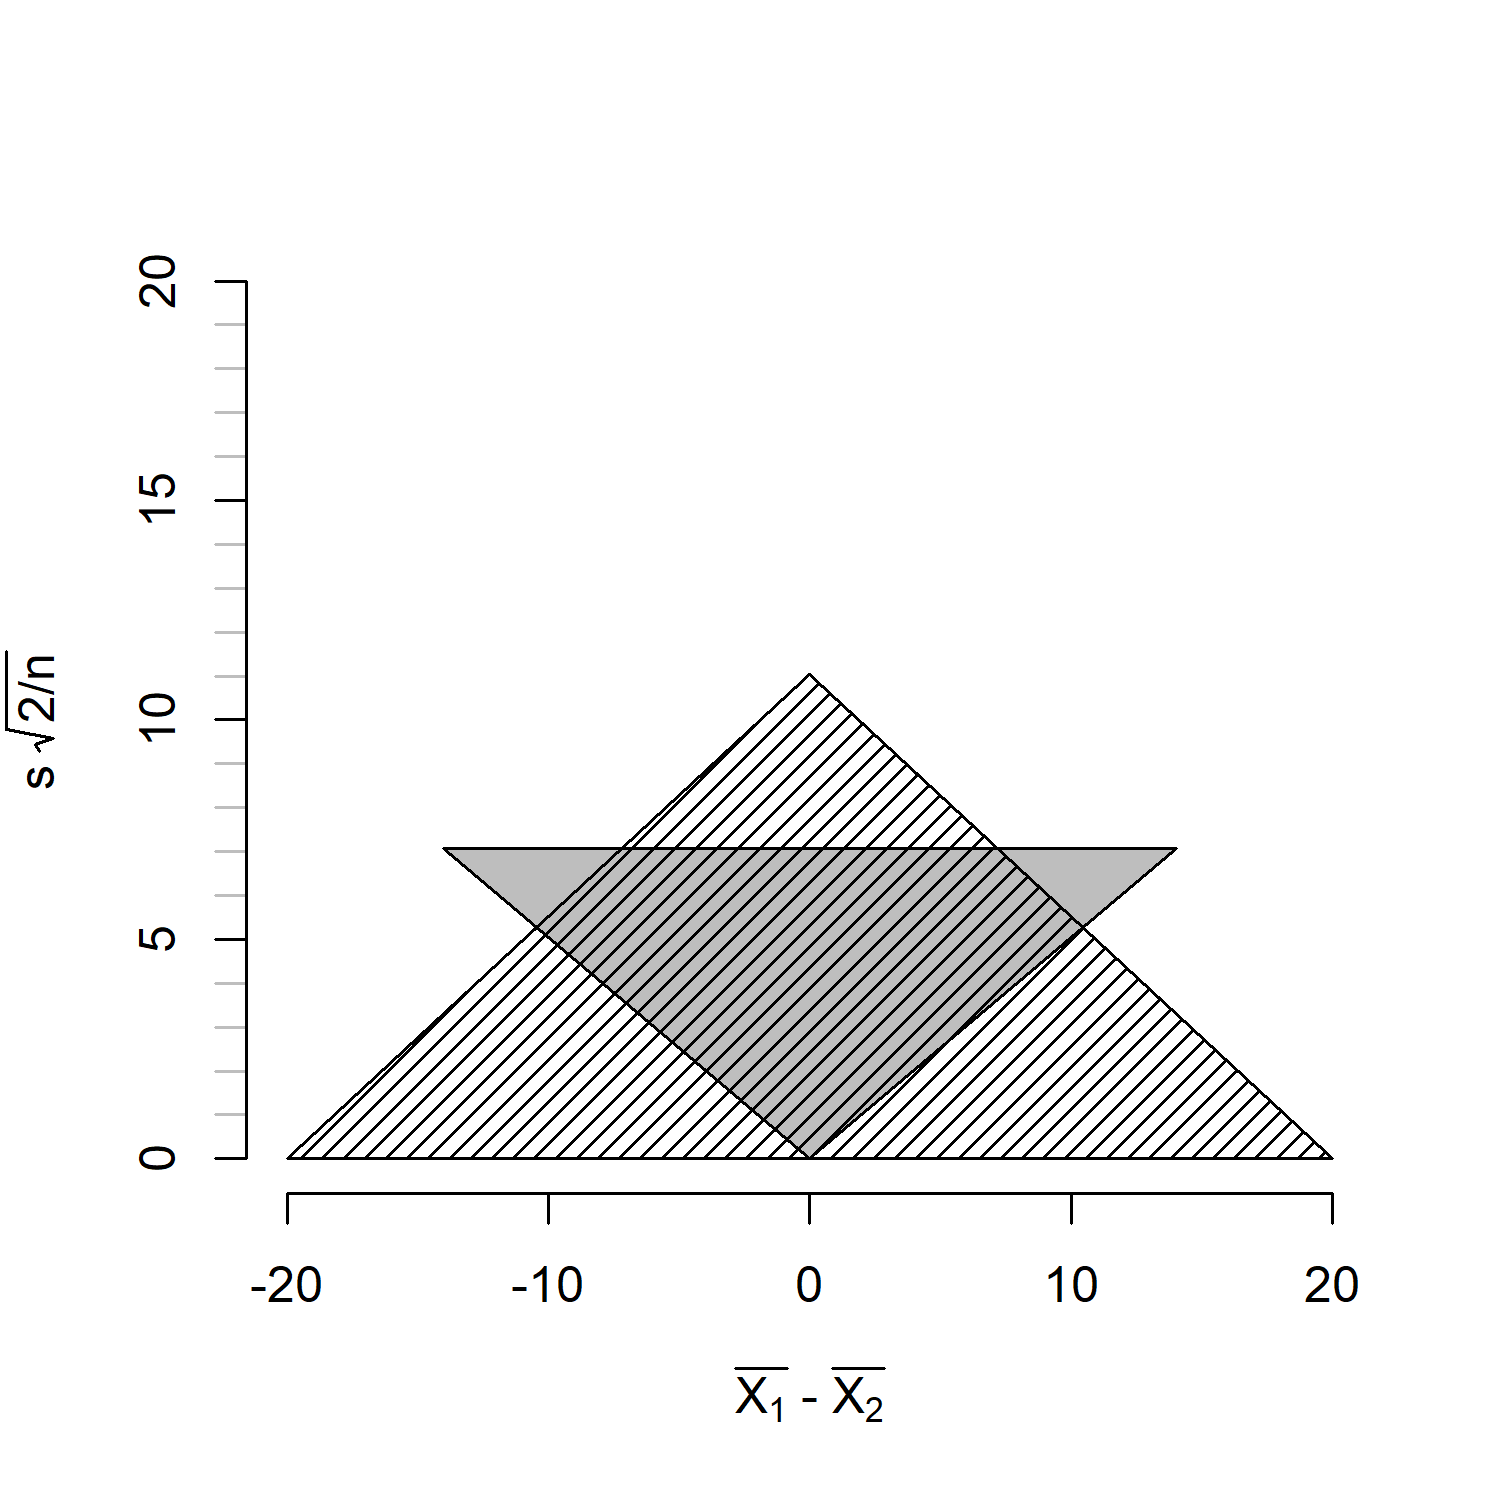
\includegraphics[width=0.4\linewidth]{C:/Users/mdelacre/Documents/Github project/thesis/Chapitre 5/Illustration/Fig1} 

}

\caption{Région d'équivalence pour l'approche de la puissance (zone grisée) et pour le TOST (zone hachurée), pour l'exemple où $|\theta$|=20, n = 50 et $\alpha=.05$}\label{fig:schuirman2}
\end{figure}

\hypertarget{les-tests-duxe9quivalence}{%
\subsection{Les tests d'équivalence}\label{les-tests-duxe9quivalence}}

Avec les tests d'équivalence, il n'est pas possible de démontrer qu'un effet vaille exactement zéro (\textbf{meyners\_equivalence\_2012?}). Il est par contre possible de montrer que l'effet observé est suffisamment petit pour être jugé non pertinent. Or, cela peut s'avérer précieux dans de nombreuses situations, par exemple pour justifier la décision de regrouper plusieurs groupes de sujets ensemble (\textbf{rogers\_using\_1993?}), pour contrôler qu'il n'y ait pas de différence trop importante entre les groupes sur base de critères autres que le (ou les) facteur(s) d'intérêts en cas de quasi-expérience (\textbf{seaman\_equivalence\_1998?}) ou encore pour falsifier une théorie qui prônerait en faveur d'un effet dépassant une certaine taille (\textbf{lakens\_equivalence\_2017?}; \textbf{anderson\_theres\_2016?}).

Le point de départ des tests d'équivalence est de définir \(\theta_1\) et \(\theta_2\), les bornes inférieures et supérieures de la zone d'équivalence, cette dernière contenant l'ensemble des valeurs jugées trop petites pour être susceptibles de nous intéresser. Ces bornes peuvent être exprimées soit dans l'unité des données brutes, soit en terme standardisé, mais doivent être définies avant la récolte des données (Anderson \(\&\) Maxwell, 2016; Lakens et al., 2018). Il existe ensuite plusieurs approches pour démontrer que l'effet observé se situe dans la zone d'équivalence (voir \textbf{meyners\_equivalence\_2012?}). Parmis celles-ci, une approche très simple est celle du ``Two one-sided tests'' (\textbf{schuirmann\_comparison\_1987?}; \textbf{lakens\_equivalence\_2017?}), que l'on appelle plus communément le TOST.\footnote{Il existe des alternatives au TOST qui sont très légèrement plus puissantes, mais le gain marginal en termes de puissance est contrebalancé par un niveau de complexité beaucoup plus élevé (Meyners, 2012).} Le principe est de définir deux hypothèses nulles. La première est que l'effet observé est inférieur à la borne inférieure de la zone d'équivalence : \[\it H0_1\;: \theta < \theta_1, \; avec \; \theta_1 \neq 0\] La seconde est que l'effet observé est supérieur à la borne supérieure de la zone d'équivalence : \[\it H0_2\;: \theta > \theta_2, \; avec \; \theta_2 \neq 0\] Lorsque les deux hypothèses nulles peuvent être simultanément rejetées, on peut conclure à l'équivalence (\textbf{seaman\_equivalence\_1998?}). Cela équivaut, statistiquement parlant, à montrer que l'intervalle de confiance à \((1-2\times\alpha)\%\) est entièrement inclus dans la zone d'équivalence (\textbf{seaman\_equivalence\_1998?}; \textbf{lakens\_equivalence\_2017?}). Notons qu'il n'est pas nécessaire de reporter les résultats des deux tests unilatéraux lorsqu'on réalise le TOST, il suffit de reporter les résultats du test associé à la plus petite valeur de statistique (et par conséquent, à la plus grande \(p\)-valeur). En effet, si ce test amène à conclure au rejet de l'hypothèse nulle, le second test amènera automatiquement à la même conclusion (Lakens et al., 2018; Rogers et al.,1993). Cette remarque reste vraie dans le cas particulier où les deux tests sont associés à la même valeur de statistique puisque dans ce cas, les deux tests mèneront à une conclusion identique (Rogers et al., 1993). Notons également qu'il n'est pas nécessaire de procéder à une correction du risque alpha due à la réalisation simultanée de deux tests. En effet, une erreur de type I (rejeter à tort l'hypothèse nulle) ne peut être commise que si l'hypothèse nulle est vraie. Or, les deux hypothèses nulles testées sont mutuellement exclusives : il n'est pas possible que \(\theta\) soit simultanément inférieur à \(\theta_1\) (ce qui correspond à \(\it H0_1\)) et supérieur à \(\theta_2\) (ce qui correspond à \(\it H0_2\)).

Jusqu'il y a peu, le TOST n'était pas disponible dans la plupart des logiciels, à l'exception de Minitab, ce qui constituait un frein important à son usage. Pour cette raison, (\textbf{lakens\_20\_2016?}) a créé le package R ``TOSTER'' et plus récemment encore, ce même package a été implémenté dans Jamovi.\footnote{Jamovi est un logiciel clic-bouton entièrement gratuit qui gagne en popularité et qui présente, parmi ses nombreux avantages, le fait d'être particulièrement convivial. Dans la mesure où la plupart des chercheurs sont plus enclins à utiliser des procédures si elles sont implémentées dans ce type de logiciel (Fraas $\&$ Newman, 2000), cela constitue une excellente nouvelle pour le devenir du TOST dans la recherche en psychologie.} Tant dans R que dans Jamovi, le package compare simultanément l'effet observé à l'absence d'effet (cela correspond au test traditionnel) ainsi qu'aux deux bornes de la zone d'équivalence (cela correspond au TOST). Il en découle 4 conclusions distinctes possibles (\textbf{lakens\_equivalence\_2017?}), qui sont illustrées dans la figure \ref{fig:equiv1} dans le contexte de la comparaison de deux moyennes indépendantes :

\begin{figure}

{\centering 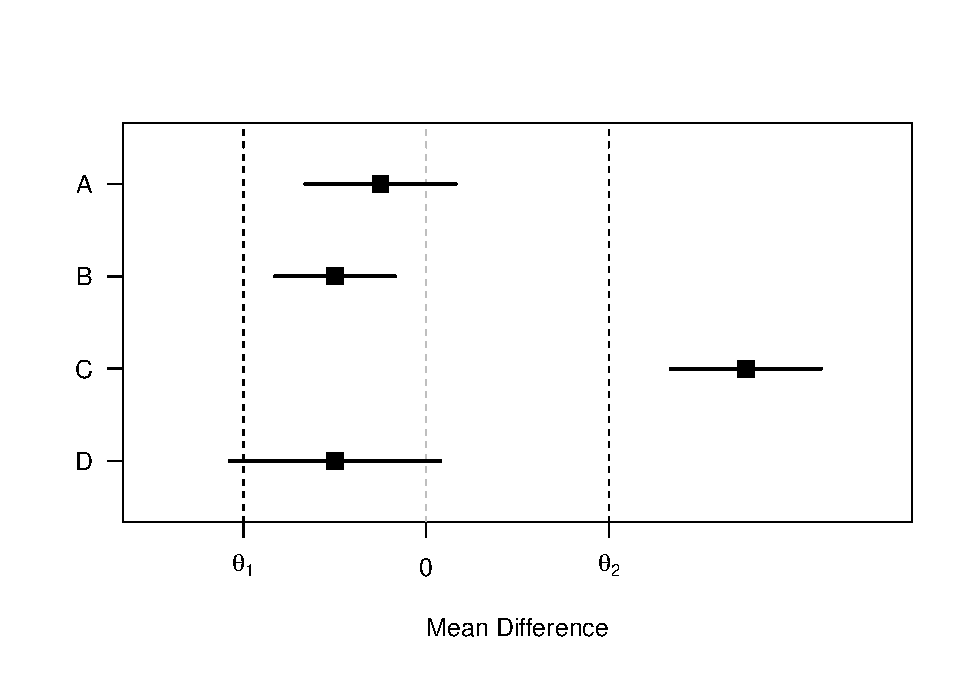
\includegraphics[width=0.8\linewidth]{chp5_format-Rmd_bib_files/figure-latex/equiv1-1} 

}

\caption{Différence de moyennes ($\bar{X_1}-\bar{X_2}$) et IC à $1-2\alpha\%$ autour de la différence de moyennes ($\bar{X_1}-\bar{X_2}$) pour 4 scénarios distincts.}\label{fig:equiv1}
\end{figure}

\begin{enumerate}
\def\labelenumi{(\arabic{enumi})}
\item
  La différence de moyenne observée diffère significativement des deux bornes d'équivalence, mais pas de 0 (scénario A, Figure \ref{fig:equiv1}) : dans ce cas, on conclura à l'absence d'un effet au moins aussi grand que les bornes d'équivalence.
\item
  La différence de moyenne observée diffère significativement des deux bornes d'équivalence ainsi que de 0 (scénario B, Figure \ref{fig:equiv1}) : on conclura alors qu'il existe un effet non nul, mais qui ne dépasse pas une certaine taille fixée par les bornes. C'est ce qui arrive typiquement lorsqu'on travaille avec de très grands échantillons, si bien que le test traditionnel est très puissant, même pour détecter des effets très petits (Rogers et al., 1993).
\item
  La différence de moyenne observée diffère significativement de 0, mais ne diffère pas significativement d'au moins une des deux bornes d'équivalence (scénario C, Figure \ref{fig:equiv1}) : on conclura alors à la présence d'un effet non nul (Rogers et al., 1993).
\item
  La différence de moyenne observée ne diffère significativement ni d'au moins une des deux bornes d'équivalence, ni de 0 (scénario D, Figure \ref{fig:equiv1}) : c'est ce qui arrive lorsque les données sont si imprécises qu'on ne peut tirer aucune conclusion. Les données semblent compatibles tant avec un effet nul qu'avec un effet supérieur au SESOI.
\end{enumerate}

\hypertarget{duxe9finir-les-bornes-de-la-zone-duxe9quivalence}{%
\subsection{Définir les bornes de la zone d'équivalence}\label{duxe9finir-les-bornes-de-la-zone-duxe9quivalence}}

L'aspect le plus compliqué dans la réalisation du TOST est la définition des bornes d'équivalence. Dans certains cas, il est possible de définir un critère objectif qui permettra de déterminer à partir de quand un effet est jugé pertinent (Lakens et al., 2018). Dans ce cas, établir l'équivalence revient à rejeter la présence d'un effet ayant un quelconque intérêt pratique (Rogers et al., 1993). Par exemple, (\textbf{burriss\_changes\_2015?}) avaient émis l'hypothèse qu'une augmentation de la rougeur de la peau chez les femmes, en période d'ovulation, les rendraient plus attractives pour les hommes. Or, une telle hypothèse n'est crédible que si le changement facial est visible à l'oeil nu. Dans ce contexte, le SESOI serait la plus petite variation dans la rougeur de la peau qu'il est possible de détecter à l'oeil nu (Lakens et al., 2018). Il est également parfois possible pour des experts de déterminer expérimentalement ce qui constitue un changement important, pour certaines échelles fréquemment utilisées en vue de mesurer des construits psychologiques. (\textbf{button\_minimal\_2015?}), par exemple, ont interrogé un grand nombre de patients dépressifs quant à leur ressenti subjectif en termes d'amélioration de leur dépression au cours d'un certain laps de temps, et ont comparé leurs réponses à la différence de scores obtenus à l'aide du BDI\footnote{Le BDI (Beck Depression Inventory) est une échelle auto-rapportée évaluant les symptômes cognitifs courants de la dépression.  Cette échelle est constituée de 21 items évalués à l'aide des échelles de Likert allant de 0 à 3, ce qui donne un score total compris entre 0 et 63 qui sera d'autant plus élevé que la dépression sera sévère (Button et al., 2015).} dans ce même laps de temps (Lakens et al., 2018). Cela leur a permis de déterminer ce qu'il considérait comme étant une différence pratiquement significative sur l'échelle du BDI. Malheureusement, il n'est pas toujours possible d'établir un critère objectif en vue de définir les bornes d'équivalence. Dans ce cas, il existe diverses stratégies, plus subjectives, en vue d'établir ces bornes. En les utilisant, il faut cependant avoir conscience du fait que la question à laquelle nous répondons varie en fonction de la stratégie utilisée.

Il est possible de déterminer des bornes en s'inspirant de balises existantes, en vue d'exclure la présence d'un effet jugé petit, moyen ou grand par ces balises (Lakens et al., 2018). Notons que si cette stratégie est tentante de par sa simplicité, elle doit être utilisée avec prudence. D'abord, un effet ne devrait être qualifié de petit, moyen ou grand qu'en comparaison à d'autres effets connus, et non sur base d'impressions qualitatives (\textbf{gignac\_effect\_2016?}). Dit autrement, il est important d'avoir un cadre de référence pour juger de la taille d'un effet. Or, les balises de Cohen (en l'occurrence, les balises les plus célèbres et les plus largement utilisées) sont dépourvues de ce cadre de référence, puisqu'elles ont été établies à une époque où très peu de chercheurs se préoccupaient de la taille des effets étudiés (\textbf{funder\_evaluating\_2019?}). Depuis Cohen, certains chercheurs ont déployé de gros efforts en vue d'établir de nouvelles normes sur base d'analyses systématiques quantitatives de la littérature. Gignac et Szodorai (2016), par exemple, ont établi de nouvelles balises pour interpréter le \(r\) de Pearson, en définissant les quartiles d'une distribution de 708 mesures dérivées de méta-analyses issues de la psychologie sociale et de la personnalité. C'est de la sorte qu'ils ont proposé d'interpréter respectivement des mesures de 0.10, 0.20 et 0.30, dans ces domaines de la psychologie, comme représentant des effets relativement petits, typiques et relativement larges. Ces normes ont également été approuvées par Funder et Ozer (2019).\footnote{Funder et Ozer (2019) ont relevé plusieurs enquêtes ayant calculé un $r$ de Pearson moyen de .21 sur base d'effets publiés dans la littérature en psychologie sociale et en psychologie de la personnalité. Par ailleurs, ils rappellent qu'en raison du biais de publication, un chercheur obtenant un $r$ de Pearson de .21 dans une nouvelle étude peut être assuré d'avoir détecté un effet plus grand que généralement trouvé.} Ensuite, les balises ne prennent pas en compte le contexte de l'étude si bien que statuer sur la taille d'un effet ne fournit pas nécessairement d'information sur sa valeur. Imaginons un antidépresseur B qui permette de réduire très légèrement les symptômes de dépression par rapport à un antidépresseur A déjà présent sur le marché et qui, en outre coûte moins cher. Même si statistiquement parlant, on observe une très faible taille d'effet, une analyse coût/bénéfice amènerait très vraisemblablement à conclure à la pertinence de cet effet. Pour cela, les balises devraient toujours être utilisées en dernier recours, lorsqu'on ne dispose d'aucune autre information (\textbf{gignac\_effect\_2016?}).

La taille des échantillons d'une étude est une information sur laquelle nous pouvons également nous baser en vue de fixer des bornes d'équivalence. Dans le contexte d'une réplication d'étude, cette information peut servir à déterminer si la puissance de l'outil utilisé par le chercheur d'origine était suffisante en vue de tester l'effet ciblé. Une stratégie proposée par Lakens et al.~(2018) consiste à définir comme borne d'équivalence le plus petit effet que l'étude d'origine aurait pu détecter comme étant significative.\footnote{Dans le contexte d'une réplication, il nous semble souvent plus logique de réaliser le test d'équivalence en unilatéral, puisque l'étude d'origine précisera généralement le sens de l'effet observé. C'est pourquoi nous parlons ici de borne d'équivalence au singulier.} Voici l'idée sous-jacente : idéalement, les chercheurs devraient toujours spécifier ce qu'ils considèrent comme étant le plus petit effet d'intérêt mais cette pratique n'est pas encore commune. Heureusement, même lorsqu'un auteur ne statue pas explicitement sur ce qu'il considère comme étant un effet pertinent, la taille des échantillons qu'il utilise aura un impact sur la taille des effets qu'il sera capable de mettre en évidence (en effet, plus les échantillons sont petits, plus l'effet observé doit être grand pour pouvoir être détecté comme étant significatif). Imaginons par exemple qu'un chercheur compare les moyennes de deux groupes de 30 sujets à l'aide d'un test \(t\) de Student (par facilité, considérons les conditions d'application de ce test comme étant toutes respectées). Avec ces tailles d'échantillon, il conclura au rejet de l'hypothèse nulle si la statistique \(t\) de Student vaut au minimum 2.00. Compte tenu de la relation directe entre la statistique \(t\) de Student et le \(d\) de Cohen (voir chapitre 4), on en déduit qu'il conclura au rejet de l'hypothèse nulle si le \(d\) de Cohen est supérieur ou égal à 0.52. Si l'on fixe 0.52 comme borne d'équivalence, et que l'on démontre lors d'une réplication que l'effet observé est significativement inférieur à cette borne, on suspectera que l'étude d'origine n'aurait pu détecter proprement l'effet qu'elle prétendait détecter. Une autre stratégie, proposée par (\textbf{simonsohn\_p-curve\_2014?}) consiste à déterminer la taille d'effet que l'étude d'origine aurait pu détecter avec une puissance de \(33\%\), et à utiliser cette information pour définir la borne d'équivalence. Par exemple, avec une hypothèse bilatérale, un test \(t\) de Student aura une puissance de \(33\%\) pour détecter un effet de taille 0.40 avec 30 sujets par groupe (à condition que les conditions d'application du test soient toutes respectées). Si lors de la réplication, on obtient un effet significativement inférieur à 0.40, on en déduira que sur le long terme, la probabilité que l'outil d'origine puisse proprement détecter un effet de cette taille était inférieure à \(33\%\), ce qui remet sa pertinence en cause.\footnote{Bien entendu, la valeur $33\%$ a une dimension arbitraire, comme chaque fois que l'on fixe une valeur par défaut.}
Hors du contexte des réplications d'études, on peut également se baser sur la taille des échantillons que l'on est apte à collecter soi-même, en vue de déterminer si l'on dispose d'assez de ressources pour détecter un effet ciblé (Lakens et al., 2018). Par exemple, si nous sommes dans l'incapacité de collecter des échantillons de plus de 2000 personnes, il y a certains effets que nous ne pourrons jamais détecter avec une puissance suffisante. Il est possible de déterminer la taille d'effet que nous sommes certains de pouvoir détecter avec suffisamment de puissance (ou autrement dit, dans un pourcentage raisonnable de cas, sur le long terme). Si l'on utilise cette information pour fixer la (ou les) borne(s) d'équivalence et que l'on conclut effectivement à l'équivalence, le résultat sera que pour détecter proprement l'effet que nous ciblons, il est indispensable de collecter de plus grands échantillons.

\hypertarget{comparaison-du-tost-et-du-sgpv}{%
\subsection{Comparaison du TOST et du SGPV}\label{comparaison-du-tost-et-du-sgpv}}

\begin{center}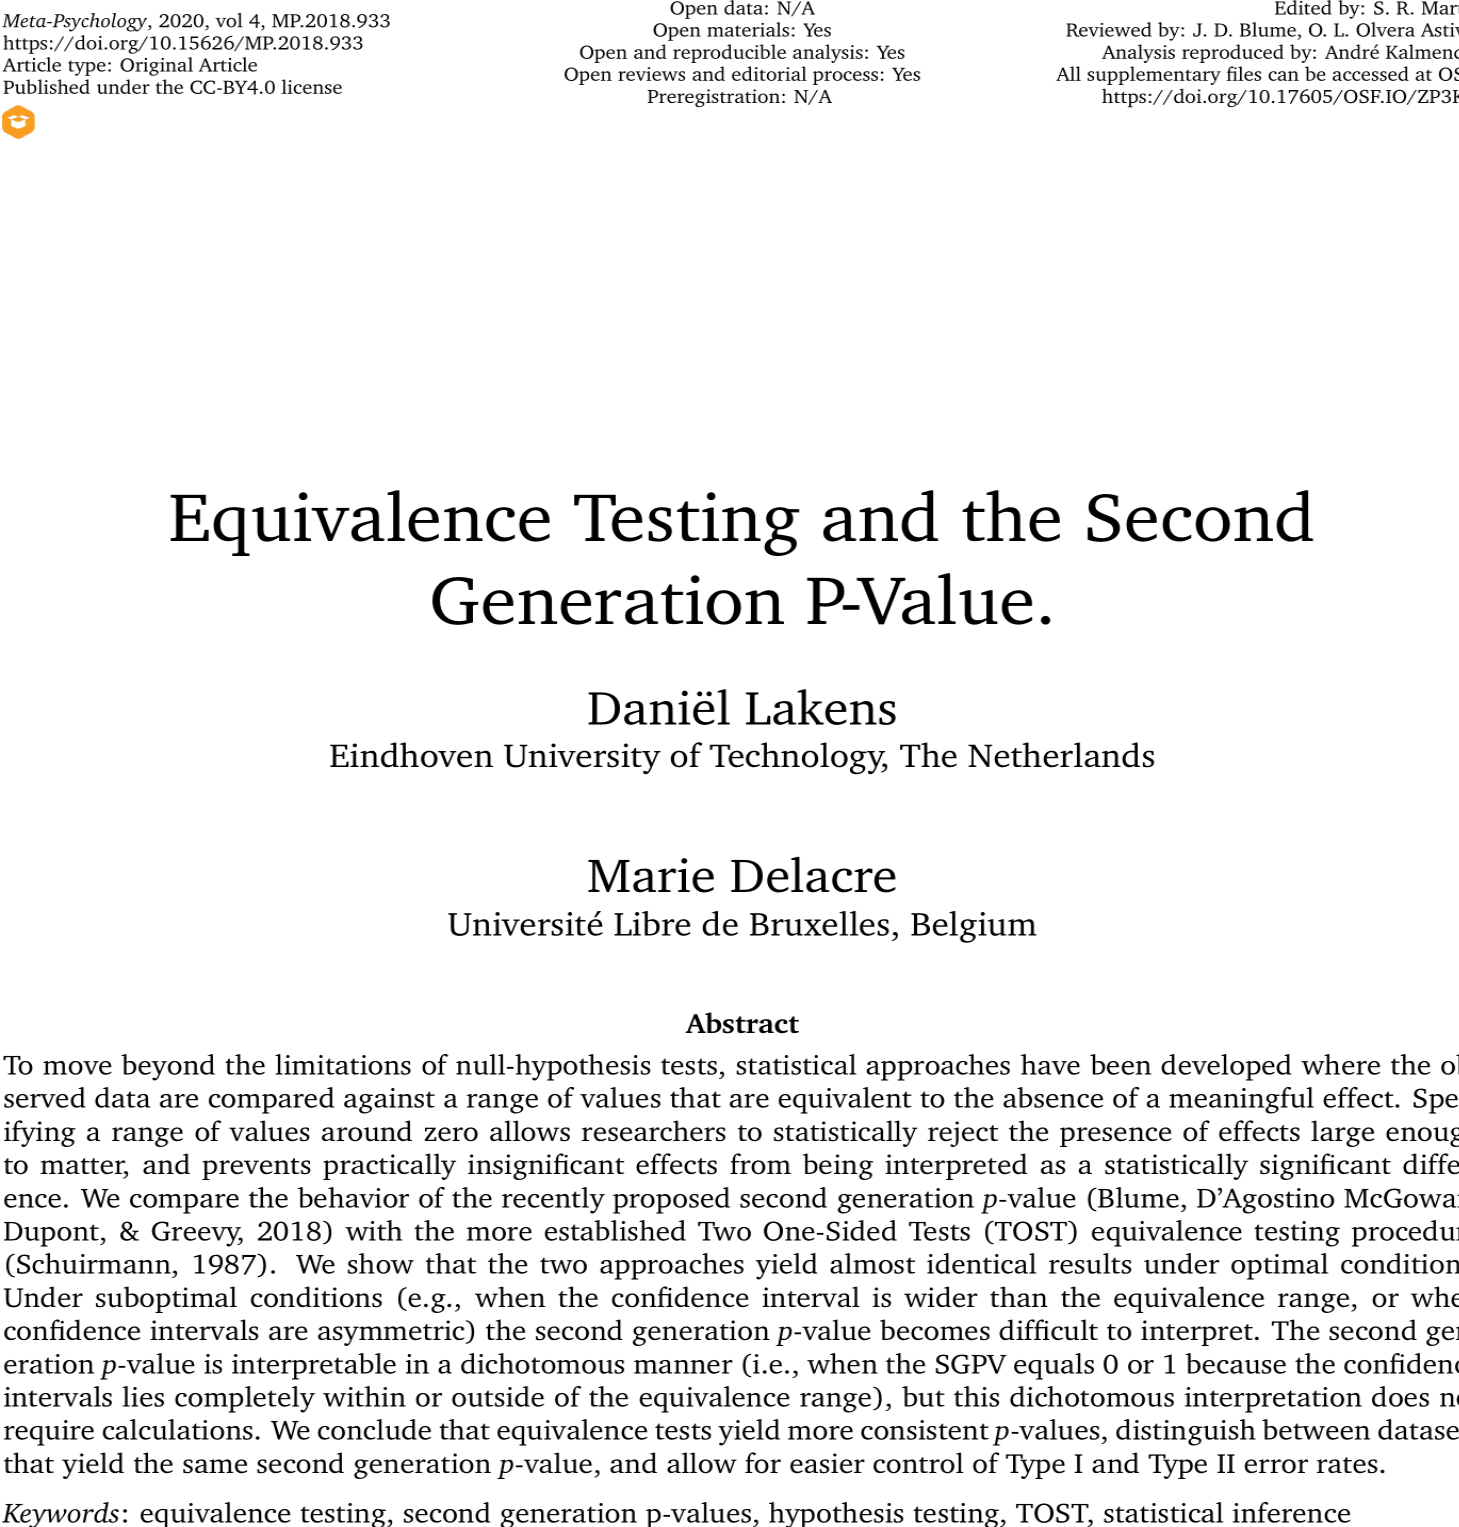
\includegraphics[height=0.7\textheight]{C:/Users/mdelacre/Documents/Github project/thesis/Chapitre 5/Chapitre 5-couverture} \end{center}
\newpage

To test predictions researchers predominantly rely on null-hypothesis tests.
This statistical approach can be used to examine whether observed data are sufficiently surprising under the null hypothesis to reject an effect that equals exactly zero.
Null-hypothesis tests have an important limitation, in that this procedure can only reject the hypothesis that there is no effect, while scientists should also be able to provide statistical support for \emph{equivalence}.
When testing for equivalence researchers aim to examine whether an observed effect is too small to be considered meaningful, and therefore is practically equivalent to zero.
By specifying a range around the null hypothesis of values that are deemed practically equivalent to the absence of an effect (i.e., 0 ± 0.3) the observed data can be compared against an \emph{equivalence range} and researchers can test if a meaningful effect is absent (\textbf{hauck\_new\_1984?}; \textbf{kruschke\_rejecting\_2018?}; \textbf{rogers\_using\_1993?}; \textbf{serlin\_rationality\_1985?}; \textbf{spiegelhalter\_bayesian\_1994?}; \textbf{wellek\_testing\_2010?}; \textbf{westlake\_use\_1972?}).

Second generation \emph{p}-values (SGPV) were recently proposed as a statistic that represents `the proportion of data-supported hypotheses that are also null hypotheses' (\textbf{blume\_second-generation\_2018?}).
The researcher specifies an equivalence range around a null hypothesis of values that are considered practically equivalent to the null hypothesis.
The SGPV measures the degree to which a set of data-supported parameter values falls within the interval null hypothesis.
If the estimation interval falls completely within the equivalence range, the SGPV is 1.
If the confidence interval falls completely outside of the equivalence range, the SGPV is 0. Otherwise the SGPV is a value between 0 and 1 that expresses the overlap of data-supported hypotheses and the equivalence range.
When calculating the SGPV the set of data-supported parameter values can be represented by a confidence interval (CI), although one could also choose to use credible intervals or Likelihood support intervals (SI).
When a confidence interval is used, the SGPV and equivalence tests such as the Two One-Sided Tests (TOST) procedure (\textbf{lakens\_equivalence\_2017?}; \textbf{meyners\_equivalence\_2012?}; \textbf{quertemont\_how\_2011?}; \textbf{schuirmann\_comparison\_1987?}) appear to have close ties, because both tests compare a confidence interval against an equivalence range.
Here, we aim to examine the similarities and differences between the TOST procedure and the SGPV.
We limit our analysis to continuous data sampled from a bivariate normal distribution.

The TOST procedure also relies on the confidence interval around the effect.
In the TOST procedure the data are tested against the lower equivalence bound in the first one-sided test, and against the upper equivalence bound in the second one-sided test (\textbf{lakens\_equivalence\_2018?}). For an excellent discussion of the strengths and weaknesses of different frequentist equivalence tests, including alternatives to the TOST procedure, see (\textbf{meyners\_equivalence\_2012?}).
If both tests statistically reject an effect as extreme or more extreme than the equivalence bound, you can conclude the observed effect is practically equivalent to zero from a Neyman-Pearson approach to statistical inferences.
Because one-sided tests are performed, one can also conclude equivalence by checking whether the 1-2\(\times\)\(\alpha\) confidence interval (e.g., when the alpha level is 0.05, a 90\(\%\) CI) falls completely within the equivalence bounds. Because both equivalence tests as the SGPV are based on whether and how much a confidence interval overlaps with equivalence bounds, it seems worthwhile to compare the behavior of the newly proposed SGPV to equivalence tests to examine the unique contribution of the SGPV to the statistical toolbox.

\hypertarget{the-relationship-between-p-values-from-tost-and-sgpv-when-confidence-intervals-are-symmetrical}{%
\subsubsection{\texorpdfstring{The relationship between \emph{p}-values from TOST and SGPV when confidence intervals are symmetrical}{The relationship between p-values from TOST and SGPV when confidence intervals are symmetrical}}\label{the-relationship-between-p-values-from-tost-and-sgpv-when-confidence-intervals-are-symmetrical}}

The second generation \emph{p}-value (SGPV) is calculated as:
\[
  p _ { \delta } = \frac { \left| I \cap H _ { 0 } \right| } { | I | } \times \max \left\{ \frac { | I | } { 2 \left| H _ { 0 } \right| } , 1 \right\}
\]
where I is the interval based on the data (e.g., a 95\(\%\) confidence interval) and H\textsubscript{0} is the equivalence range. The first term of this formula implies that the second generation \emph{p}-value is the width of the confidence interval that overlaps with the equivalence range, divided by the total width of the confidence interval. The second term is a `small sample correction' (which will be discussed later) that comes into play whenever the confidence interval is more than twice as wide as the equivalence range.
To examine the relation between the TOST \emph{p}-value and the SGPV we can calculate both statistics across a range of observed effect sizes. Building on the example by (\textbf{blume\_second-generation\_2018?}), in Figure \ref{fig:TOSTSGPV1} \emph{p}-values are plotted for the TOST procedure and the SGPV. The statistics are calculated for hypothetical one-sample \emph{t}-tests for observed means ranging from 140 to 150 (on the x-axis). The equivalence range is set to 145 ± 2 (i.e., an equivalence range from 143 to 147), the observed standard deviation is assumed to be 2, and the sample size is 30. For example, for the left-most point in Figure \ref{fig:TOSTSGPV1} the SGPV and the TOST \emph{p}-value is calculated for a hypothetical study with a sample size of 30, an observed standard deviation of 2, and an observed mean of 140, where the \emph{p}-value for the equivalence test is 1, and the SGPV is 0.

\begin{figure}

{\centering 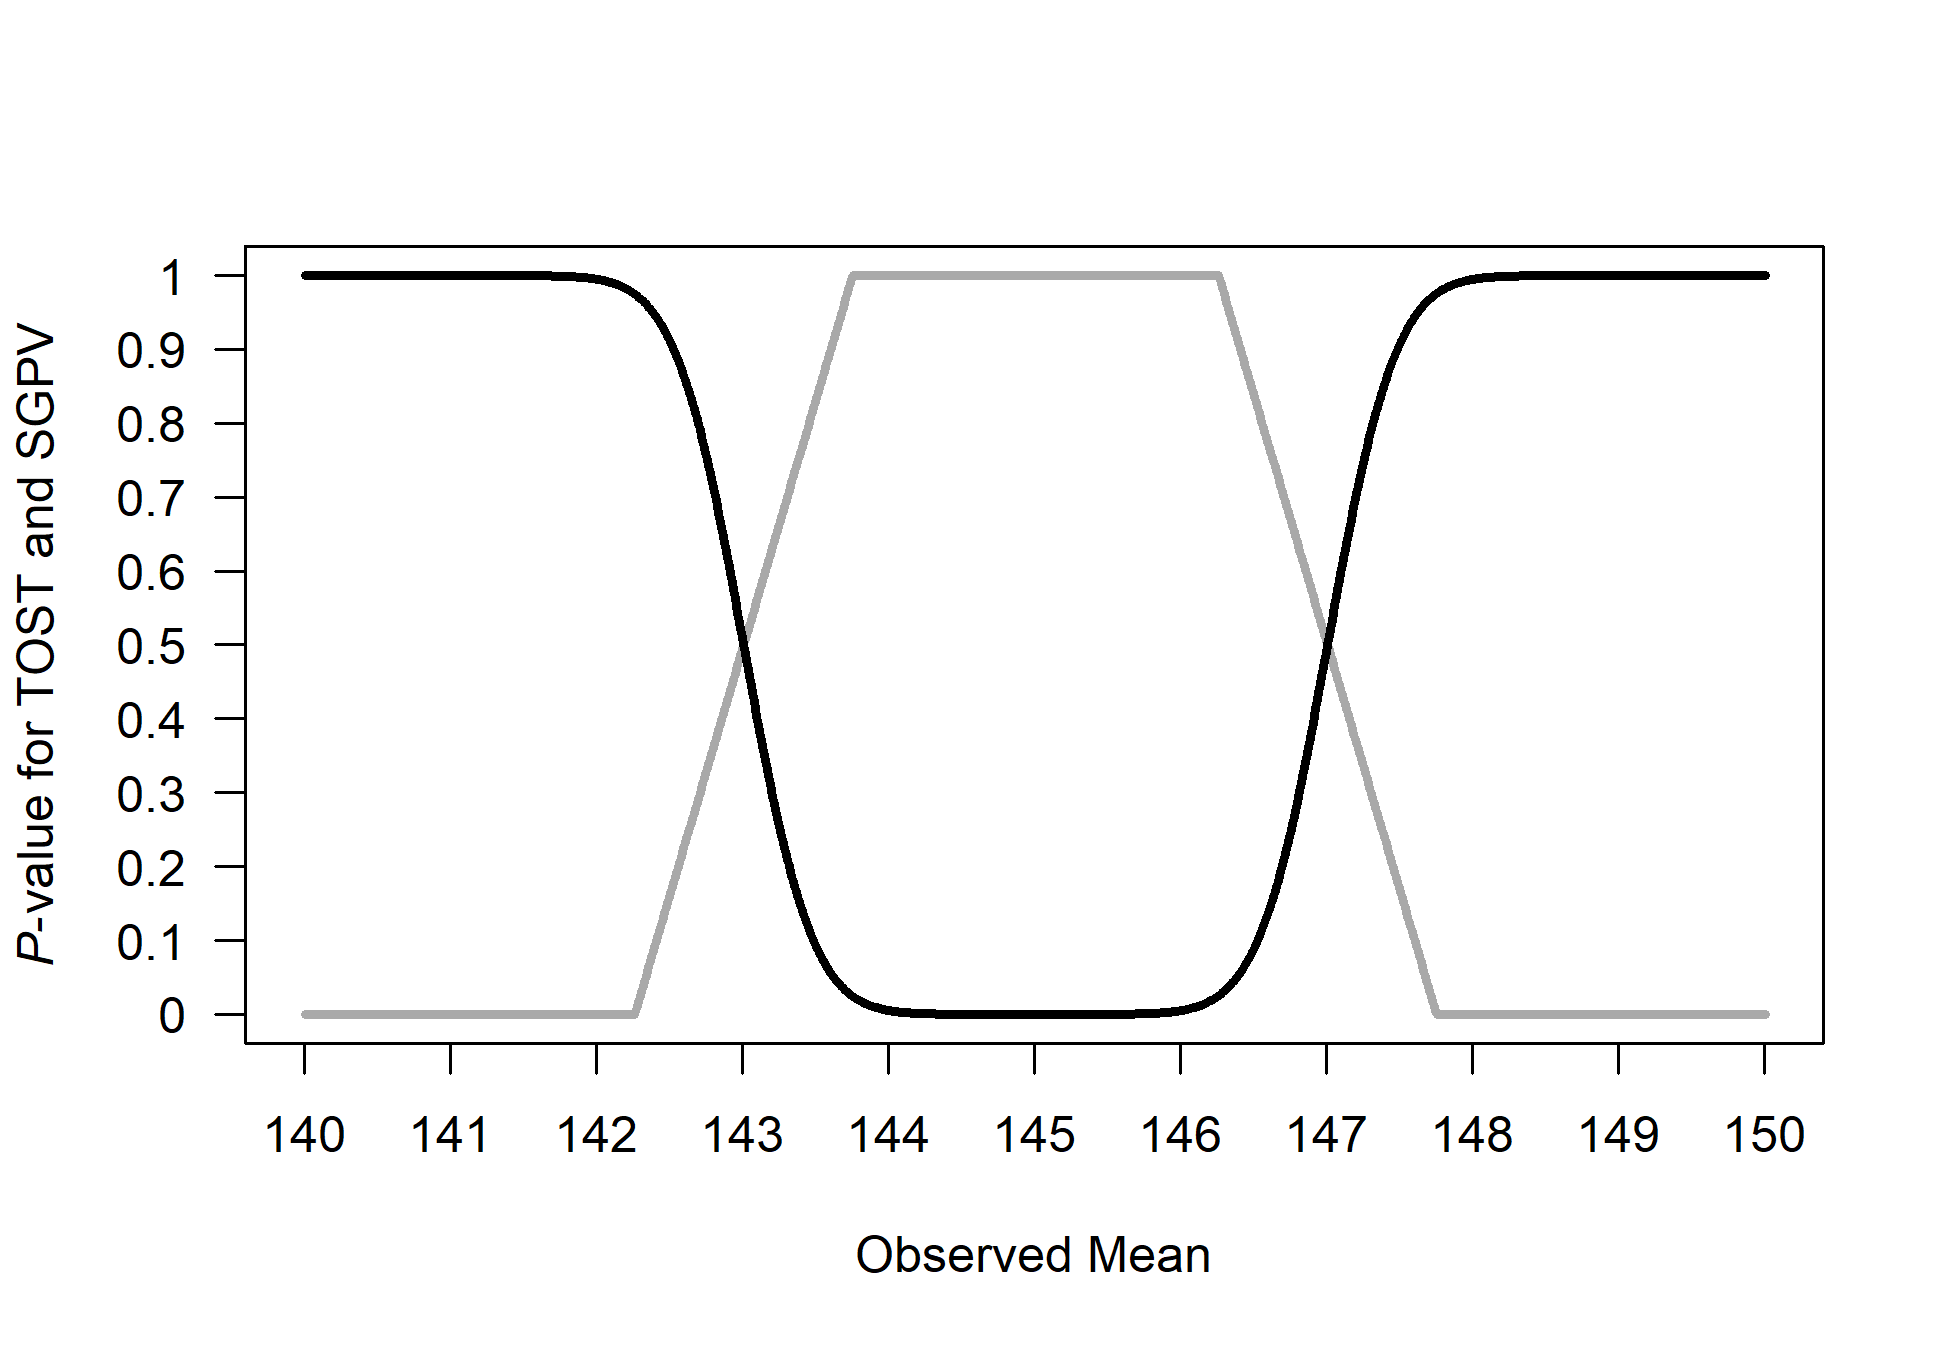
\includegraphics[height=0.94\textheight]{chp5_format-Rmd_bib_files/figure-latex/TOSTSGPV1-1} 

}

\caption{Comparison of $p$-values from TOST (black line) and SGPV (grey line) across a range of observed sample means ($x$-axis) tested against a mean of 145 in a one-sample $t$-test with a sample size of 30 and a standard deviation of 2, illustrating that when the TOST $p$-value = 0.5, the SGPV = 0.5, when the TOST $p$-value is 0.975, 1-SGPV = 1, and when the TOST $p$-value = 0.025, 1-SGPV = 0.}\label{fig:TOSTSGPV1}
\end{figure}

Our conclusions about the relationship between TOST \emph{p}-values and SGPV hold for second generation \emph{p}-values calculated from confidence intervals, and assuming data is sampled from a bivariate normal distribution. Readers can explore the relationship between TOST \emph{p}-values and SGPV for themselves in an online Shiny app : \url{http://shiny.ieis.tue.nl/TOST_vs_SGPV/}.

The SGPV treats the equivalence range as the null-hypothesis, while the TOST procedure treats the values outside of the equivalence range as the null-hypothesis. For ease of comparison we can plot 1-SGPV (see Figure \ref{fig:TOSTSGPV2}) to make the values more easily comparable. We see that the \emph{p}-value from the TOST procedure and the SGPV follow each other closely. When we discuss the relationship between the \emph{p}-values from TOST and the SGPV, we focus on their correspondence at three values, namely where the TOST \emph{p} = 0.025 and SGPV is 1, where the TOST \emph{p} = 0.5 and SGPV = 0.5, and where the TOST \emph{p} = 0.975 and SGPV = 1. These three values are important for the SGPV because they indicate the values at which the SGPV indicates the data should be interpreted as compatible with the null hypothesis (SGPV = 1), or with the alternative hypothesis (SGPV = 0), or when the data are strictly inconclusive (SGPV = 0.5). These three points of overlap are indicated by the horizontal dotted lines in Figure \ref{fig:TOSTSGPV2} at TOST \emph{p}-values of 0.975, 0.5, and 0.025.

\begin{figure}

{\centering 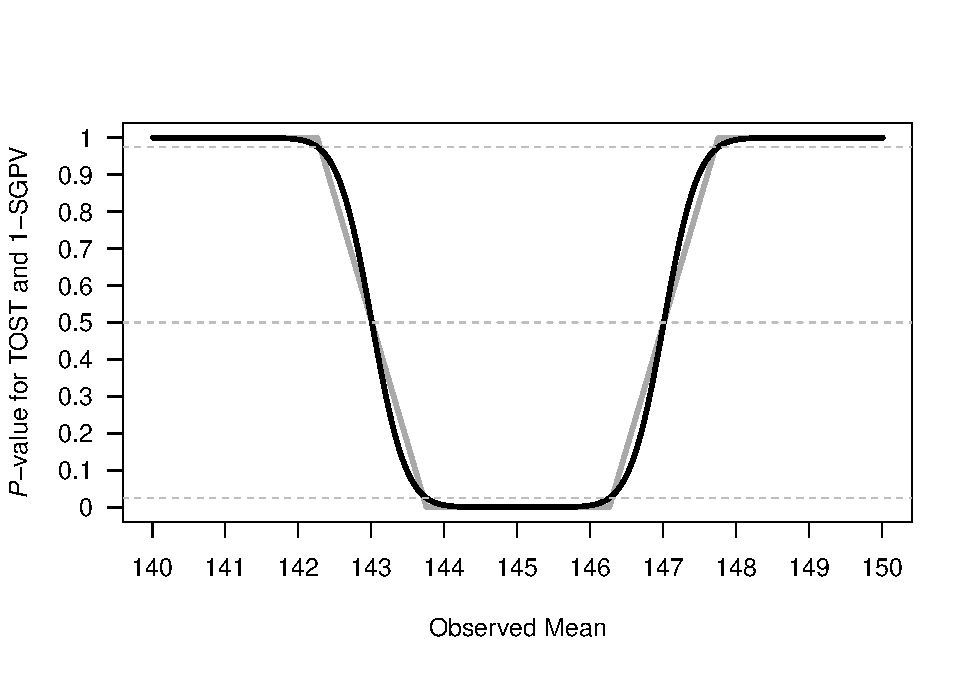
\includegraphics[height=0.94\textheight]{chp5_format-Rmd_bib_files/figure-latex/TOSTSGPV2-1} 

}

\caption{Comparison of $p$-values from TOST (black line) and 1-SGPV (grey line) across a range of observed sample means (x-axis) tested against a mean of 145 in a one-sample $t$-test with a sample size of 30 and a standard deviation of 2.}\label{fig:TOSTSGPV2}
\end{figure}

When the observed sample mean is 145, the sample size is 30, and the standard deviation is 2, and we are testing against equivalence bounds of 143 and 147 using the TOST procedure for a one-sample \emph{t}-test, the equivalence test is significant, \emph{t}(29) = 5.48, \emph{p} \textless{} .001. Because the 95\(\%\) CI falls completely within the equivalence bounds, the SGPV is 1 (see Figure \ref{fig:TOSTSGPV1}).
On the other hand, when the observed mean is 140, the equivalence test is not significant (the observed mean is far outside the equivalence range of 143 to 147), \emph{t}(29) = -8.22, \emph{p} = 1 (or more accurately, \emph{p} \textgreater{} .999 as \emph{p}-values are bounded between 0 and 1). Because the 95\(\%\) CI falls completely outside the equivalence bounds, the SGPV is 0 (see Figure \ref{fig:TOSTSGPV1}).

\hypertarget{sgpv-as-a-uniform-measure-of-overlap}{%
\paragraph{SGPV as a uniform measure of overlap}\label{sgpv-as-a-uniform-measure-of-overlap}}

It is clear the SGPV and the \emph{p}-value from TOST are closely related. When confidence intervals are symmetric we can think of the SGPV as a straight line that is directly related to the \emph{p}-value from an equivalence test for three values. When the TOST \emph{p}-value is 0.5, the SGPV is also 0.5 (note that the reverse is not true). The SGPV is 50\(\%\) when the observed mean falls exactly on the lower or upper equivalence bound, because 50\(\%\) of the symmetrical confidence interval overlaps with the equivalence range. When the observed mean equals the equivalence bound, the difference between the mean in the data and the equivalence bound is 0, the \emph{t}-value for the equivalence test is also 0, and thus the \emph{p}-value is 0.5 (situation A, Figure \ref{fig:TOSTSGPV3}).

\begin{figure}

{\centering 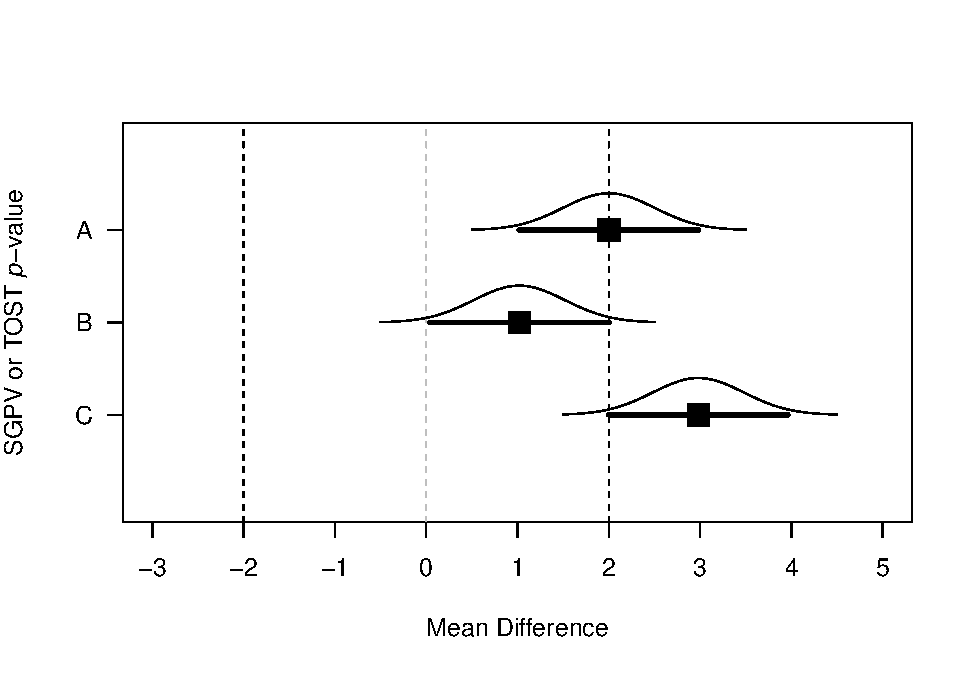
\includegraphics[height=0.94\textheight]{chp5_format-Rmd_bib_files/figure-latex/TOSTSGPV3-1} 

}

\caption{Means, normal distribution, and 95$\%$ CI for three example datasets that illustrate the relationship between $p$-values from TOST and SGPV.}\label{fig:TOSTSGPV3}
\end{figure}

Two other points always have to overlap. When the 95\(\%\) CI falls completely inside the equivalence region, and one endpoint of the confidence interval is exactly equal to one of the equivalence bounds (see situation B in Figure \ref{fig:TOSTSGPV3}) the TOST \emph{p}-value (which relies on a one-sided test) is always 0.025, and the SGPV is 1. Note that when sample sizes are small or equivalence bounds are narrow, small \emph{p}-values for the TOST or a SGPV = 1 might not be observed in practice if too few observations are collected. The third point where the SGPV and the \emph{p}-value from the TOST procedure should overlap is where the 95\(\%\) CI falls completely outside of the equivalence range, but one endpoint of the confidence interval is equal to the equivalence bound (see situation C in Figure \ref{fig:TOSTSGPV3}), when the \emph{p}-value will always be 0.975, and the SGPV is 0. Note that this situation is in essence a minimum-effect test (\textbf{murphy\_statistical\_2014?}). The goal of a minimum-effect is not just to reject a difference of zero, but to reject the smallest effect size of interest (i.e., the equivalence bounds). An equivalence test and minimum effect test against the same equivalence bound are complementary, and when a TOST \emph{p}-value is larger than 0.975, the \emph{p}-value for the minimum effect test is smaller than 0.05 (and therefore the minimum effect test provides no additional information that can not be derived from the \emph{p}-value from the equivalence test). The SGPV summarizes the information from an equivalence test (and the complementary minimum-effect test). These can be two relevant questions to ask, although it often makes sense to combine an equivalence test and a null-hypothesis test instead (\textbf{lakens\_equivalence\_2018?}).

\begin{figure}

{\centering 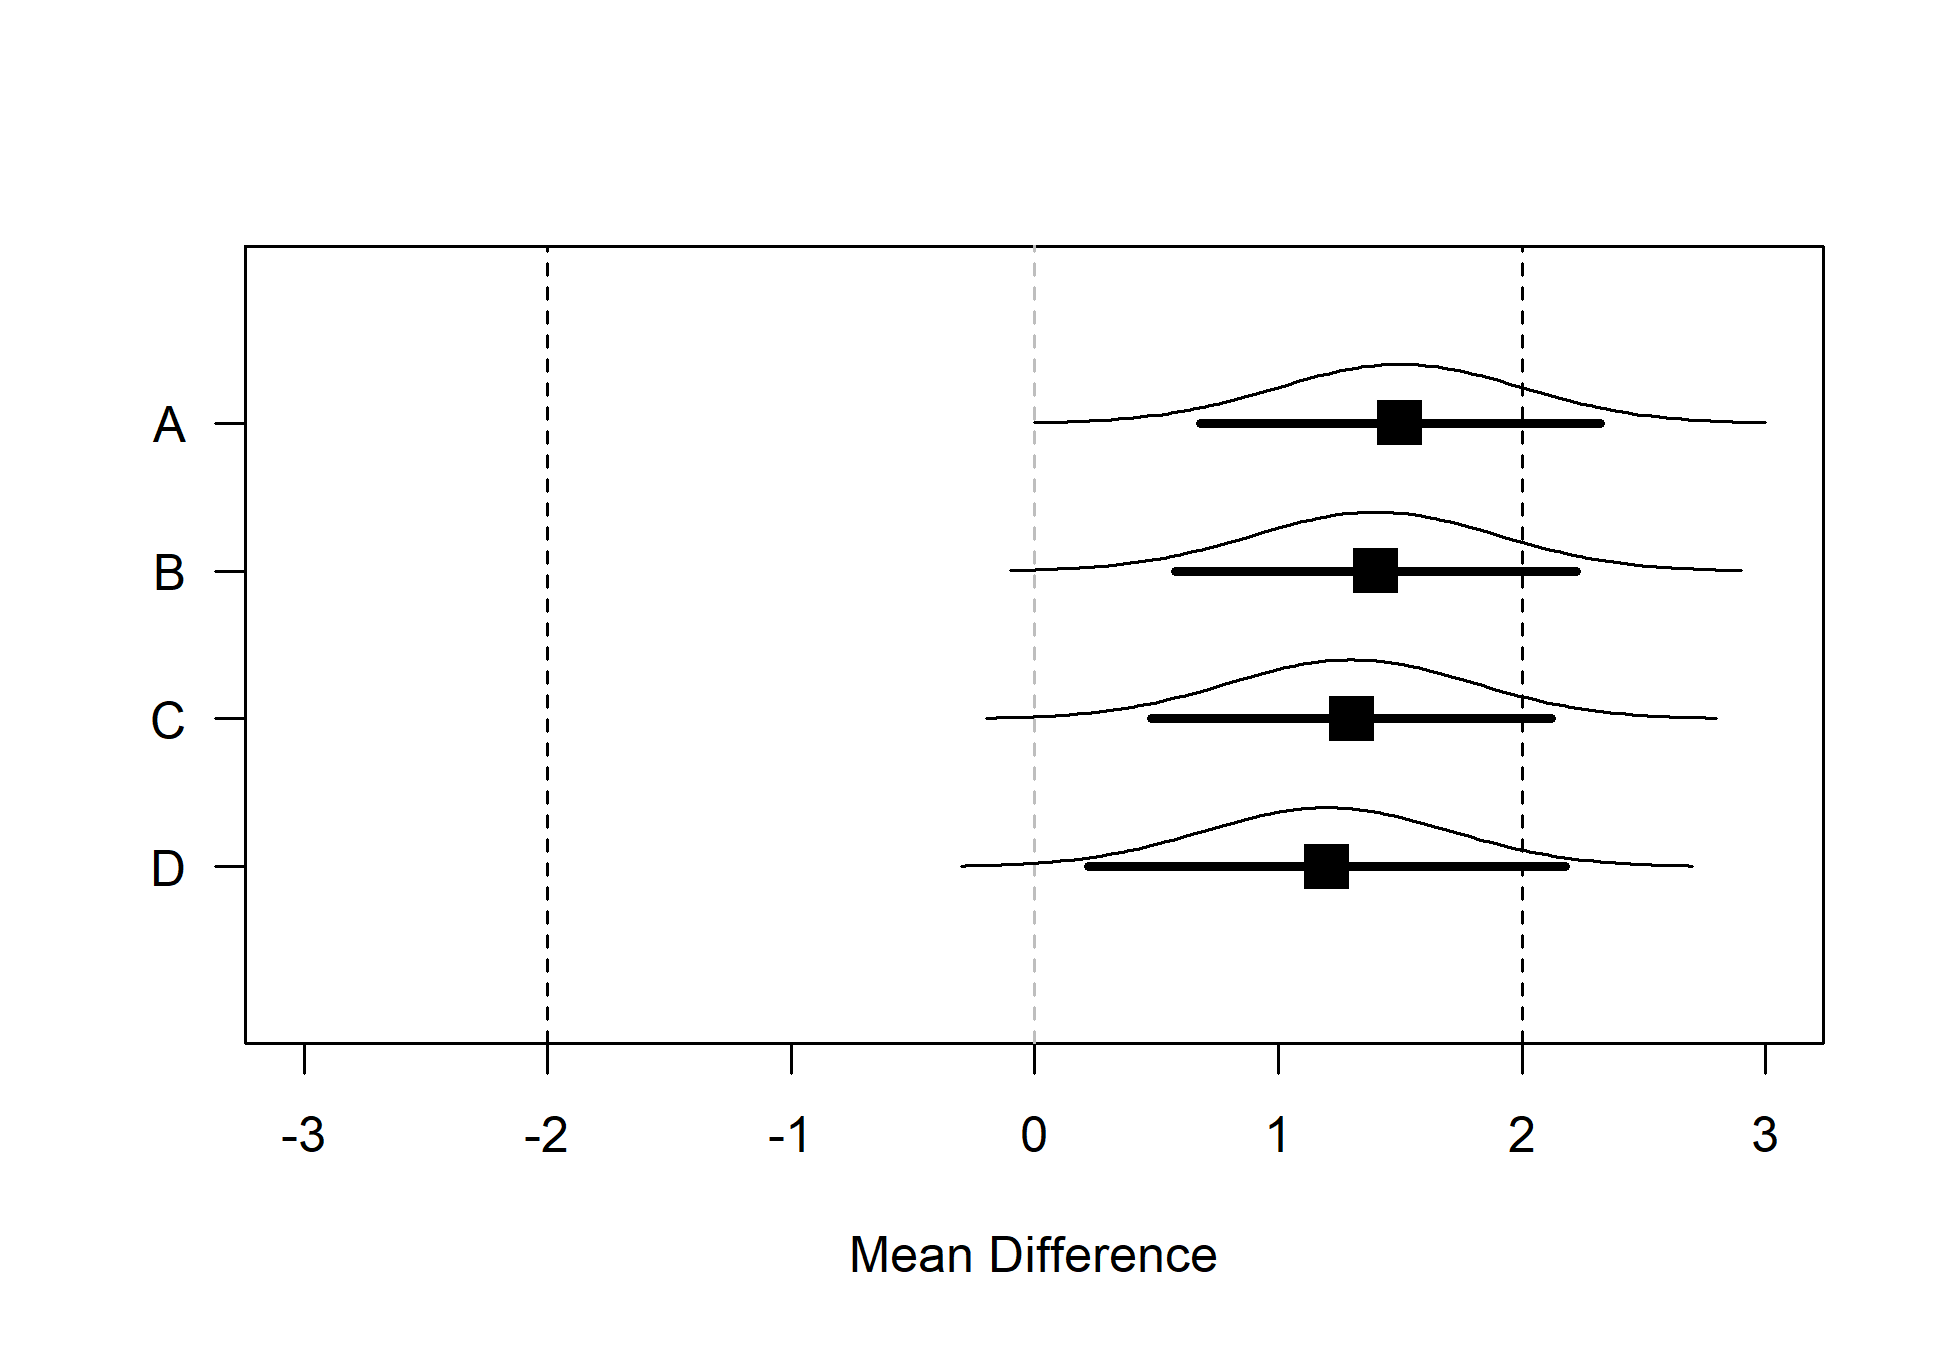
\includegraphics[height=0.94\textheight]{chp5_format-Rmd_bib_files/figure-latex/TOSTSGPV4-1} 

}

\caption{Means, normal distribution, and 95$\%$ CI for samples where the observed population mean is 1.5, 1.4, 1.3, and 1.2.}\label{fig:TOSTSGPV4}
\end{figure}

For example, in Figure \ref{fig:TOSTSGPV4} we have plotted four SGPV's. From A to D the SGPV is 0.76, 0.81, 0.86, and 0.91. The difference in the percentage of overlap between A and B (-0.05) is identical to the difference in the percentage of overlap between C and D as the mean gets 0.1 closer to the test value (-0.05).
As the observed mean in a one-sample \emph{t}-test lies closer to the test value, from situation A to D, the difference in the overlap changes uniformly.
As we move the observed mean closer to the test value in steps of 0.1 across A to D the \emph{p}-value calculated for normally distributed data are not uniformly distributed. The probability of observing data more extreme than the upper bound of 2 is (from A to D) 0.16, 0.12, 0.08, and 0.05. As we can see, the difference between A and B (0.04) is not the same as the difference between C and D (0.03). Indeed, the difference in \emph{p}-values is the largest as you start at \emph{p} = 0.5 (when the observed mean falls on the test value), which is why the line in Figure \ref{fig:TOSTSGPV1} is the steepest at \emph{p} = 0.5. Note that where the SGPV reaches 1 or 0, \emph{p}-values closely approximate 0 and 1, but never reach these values.

\hypertarget{when-different-p-values-for-equivalence-tests-yield-the-same-sgpv}{%
\paragraph{\texorpdfstring{When different \emph{p}-values for equivalence tests yield the same SGPV}{When different p-values for equivalence tests yield the same SGPV}}\label{when-different-p-values-for-equivalence-tests-yield-the-same-sgpv}}

There are three situations where \emph{p}-values for TOST differentiate between observed results, while the SGPV does not differentiate. The first two situations were discussed before and can be seen in Figure \ref{fig:TOSTSGPV1}. When the SGPV is either 0 or 1, \emph{p}-values from the equivalence test fall between 0.975 and 1 or between 0 and 0.025. Where the SGPV is 1 as long as the confidence interval falls completely within the equivalence bounds, the \emph{p}-value for the TOST continues to differentiate between results as a function of how far the confidence interval lies within the equivalence bounds (the further the confidence interval is from both bounds, the lower the \emph{p}-value). The easiest way to see this is by plotting the SGPV against the \emph{p}-value from the TOST procedure. The situations where the \emph{p}-values from the TOST procedure continue to differentiate based on how extreme the results are, but the SGPV is a fixed value are indicated by the parts of the curve where there are vertical straight lines at second generation \emph{p}-values of 0 and 1.

\begin{figure}

{\centering 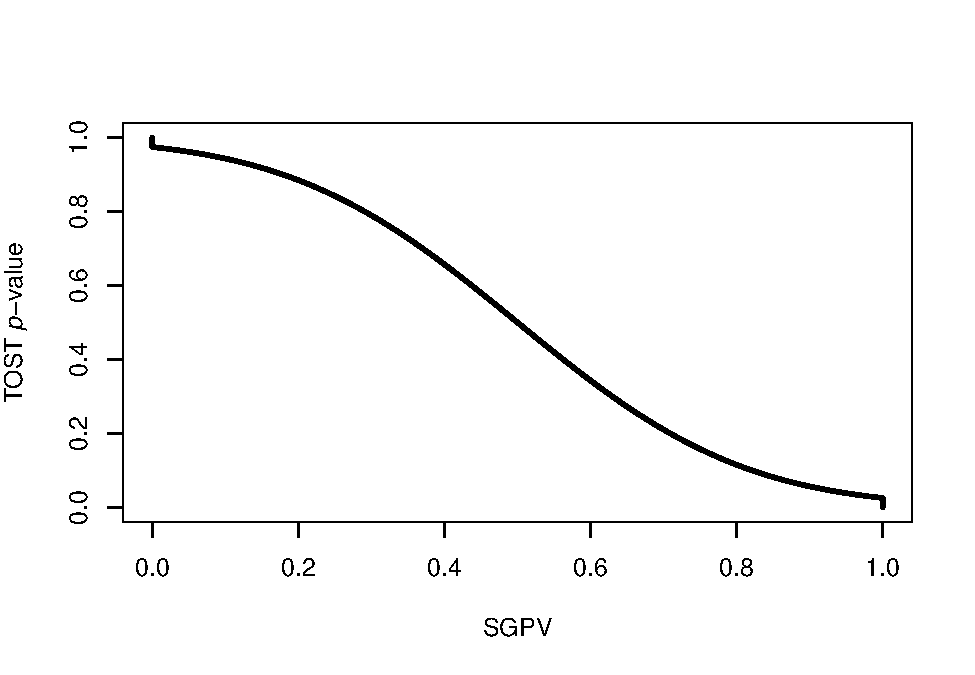
\includegraphics[height=0.94\textheight]{chp5_format-Rmd_bib_files/figure-latex/TOSTSGPV5-1} 

}

\caption{The relationship between $p$-values from the TOST procedure and the SGPV for the same scenario as in Figure \ref{fig:TOSTSGPV1}.}\label{fig:TOSTSGPV5}
\end{figure}

A third situation in which the SGPV remains stable across a range of observed effects, while the TOST \emph{p}-value continues to differentiate, is whenever the CI is wider than the equivalence range, and the CI overlaps with the upper \emph{and} lower equivalence bound. When the confidence interval is more than twice as wide as the equivalence range the SGPV is set to 0.5. (\textbf{blume\_second-generation\_2018?}) call this the `small sample correction factor.' However, it is not a correction in the typical sense of the word, since the SGPV is not adjusted to any `correct' value. When the normal calculation would be `misleading' (i.e., the SGPV would be small, which normally would suggest support for the alternative hypothesis, but at the same time all values in the equivalence range are supported), the SGPV is set to 0.5 which according to Blume and colleagues signals that the SGPV is `uninformative.' Note that the CI can be twice as wide as the equivalence range whenever the sample size is small (and the confidence interval width is large) \emph{or} when then equivalence range is narrow. It is therefore not so much a `small sample correction' as it is an exception to the typical calculation of the SGPV whenever the ratio of the confidence interval width to the equivalence range exceeds 2:1 and the CI overlaps with the upper and lower bounds.

\begin{figure}

{\centering 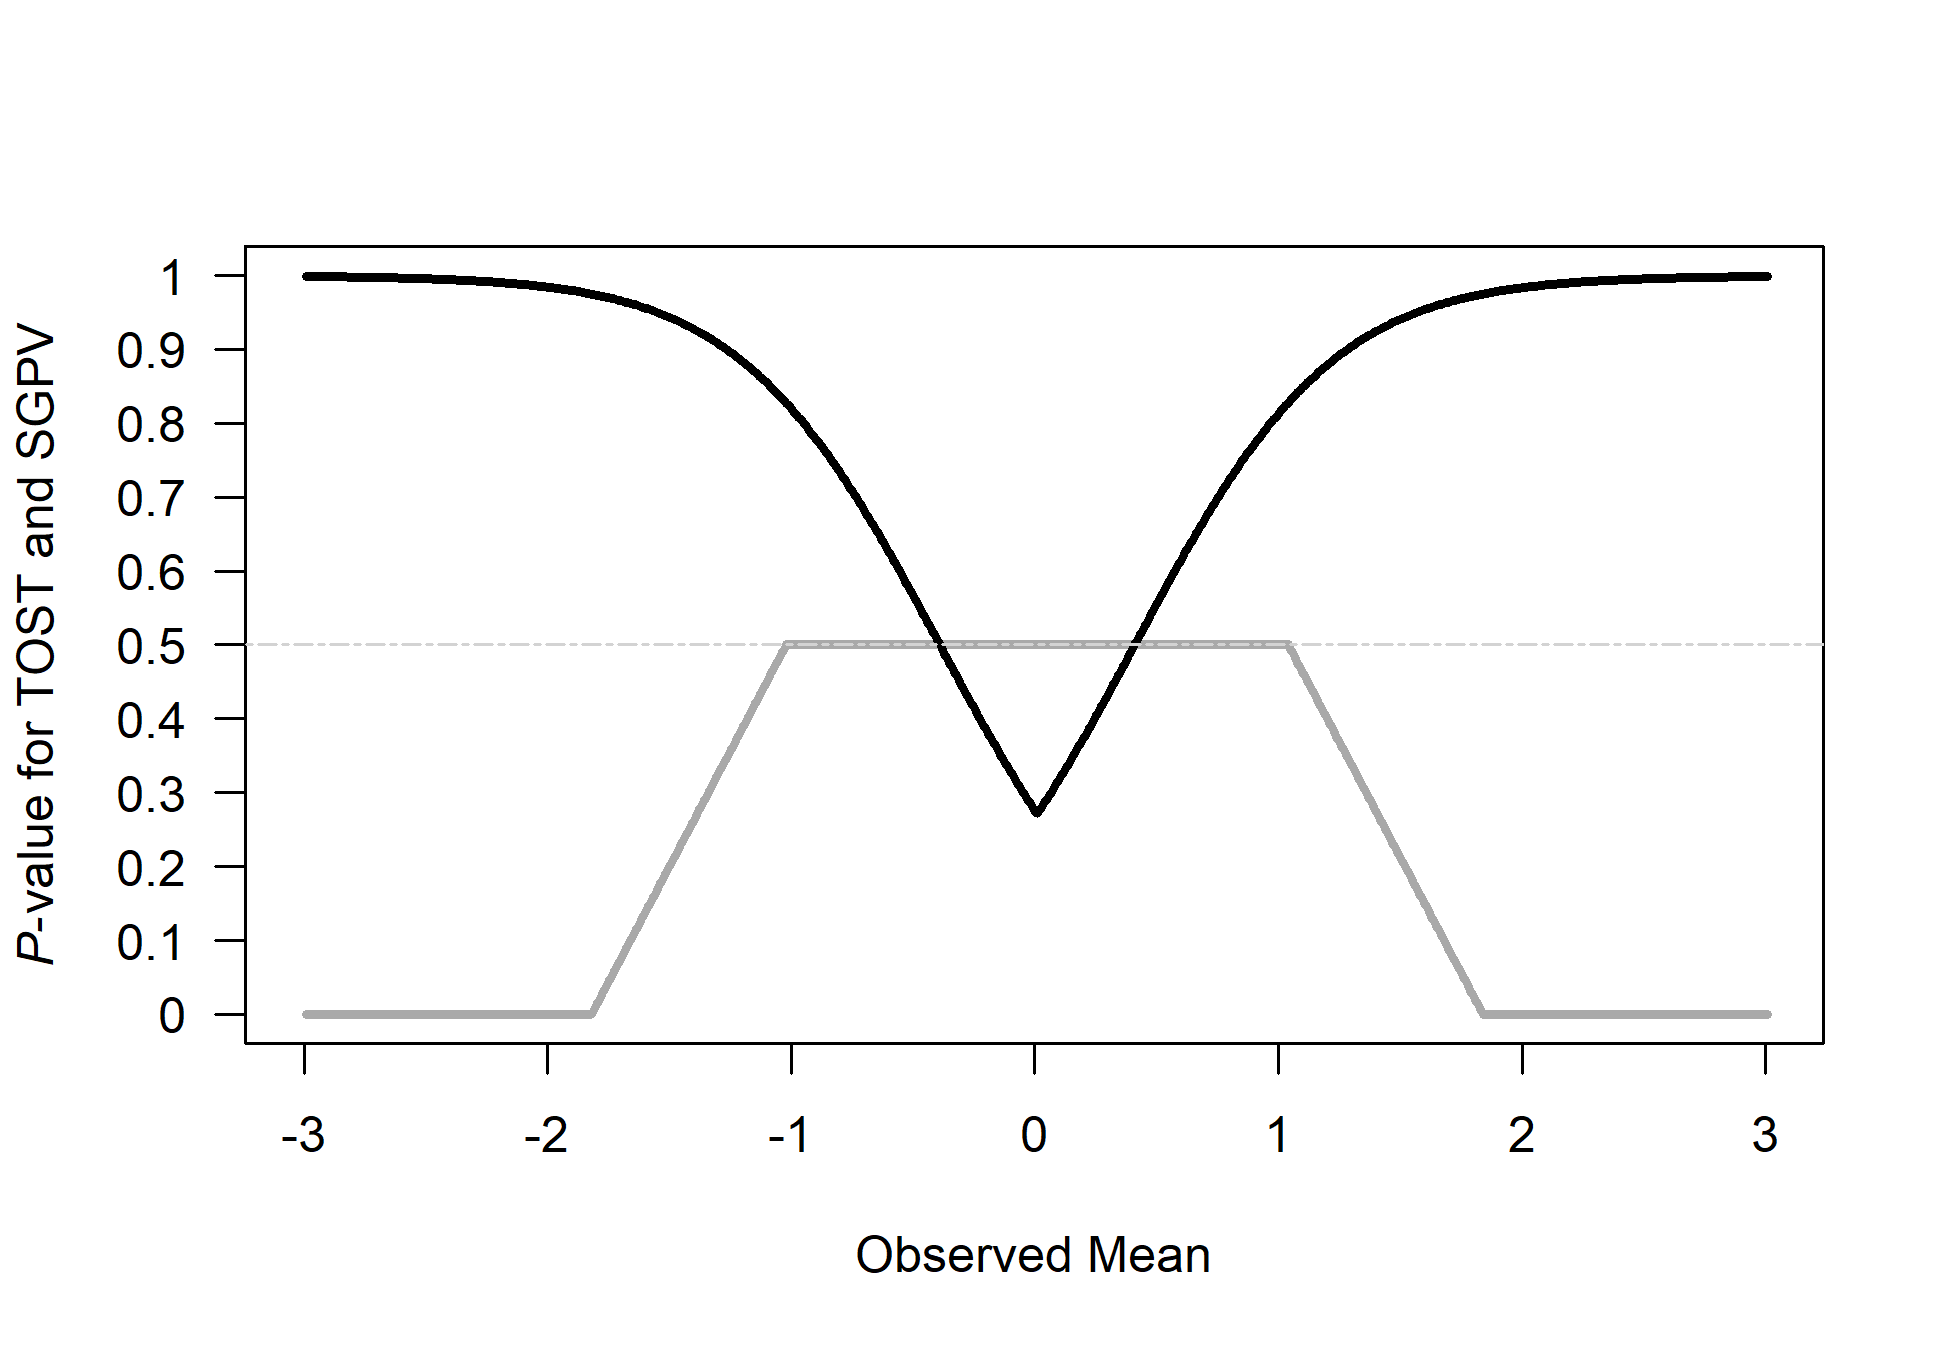
\includegraphics[height=0.94\textheight]{chp5_format-Rmd_bib_files/figure-latex/TOSTSGPV6-1} 

}

\caption{Comparison of $p$-values from TOST (black line) and SGPV (grey line) across a range of observed sample means ($x$-axis). Because the sample size is small ($n$ = 10) and with a standard deviation of 2 the CI is more than twice as wide as the equivalence range (set to -0.4 to 0.4), the SGPV is set to 0.5 (horizontal lightgrey line) across a range of observed means.}\label{fig:TOSTSGPV6}
\end{figure}

We can examine this situation by calculating the SGPV and performing the TOST for a situation where sample sizes are small and the equivalence range is narrow, such that the CI is more than twice as large as the equivalence range (see Figure \ref{fig:TOSTSGPV6}). When the two statistics are plotted against each other we can see where the SGPV is the same while the TOST \emph{p}-value still differentiates different observed means (indicated by straight lines in the curve, see Figure \ref{fig:TOSTSGPV7}). We see the SGPV is 0.5 for a range of observed means where the \emph{p}-value from the equivalence test still varies. It should be noted that in these calculations the \emph{p}-values for the TOST procedure are \emph{never} smaller than 0.05 (i.e., they do not get below 0.05 on the y-axis). In other words, we cannot conclude equivalence based on any of the observed means. This happens because we are examining a scenario where the 90\(\%\) CI is so wide that it never falls completely within the two equivalence bounds.

As (\textbf{lakens\_equivalence\_2017?}) notes : ``in small samples (where CIs are wide), a study might have no statistical power (i.e., the CI will always be so wide that it is necessarily wider than the equivalence bounds).'' None of the \emph{p}-values based on the TOST procedure are below 0.05, and thus, in the long run we have 0\(\%\) power.

\begin{figure}

{\centering 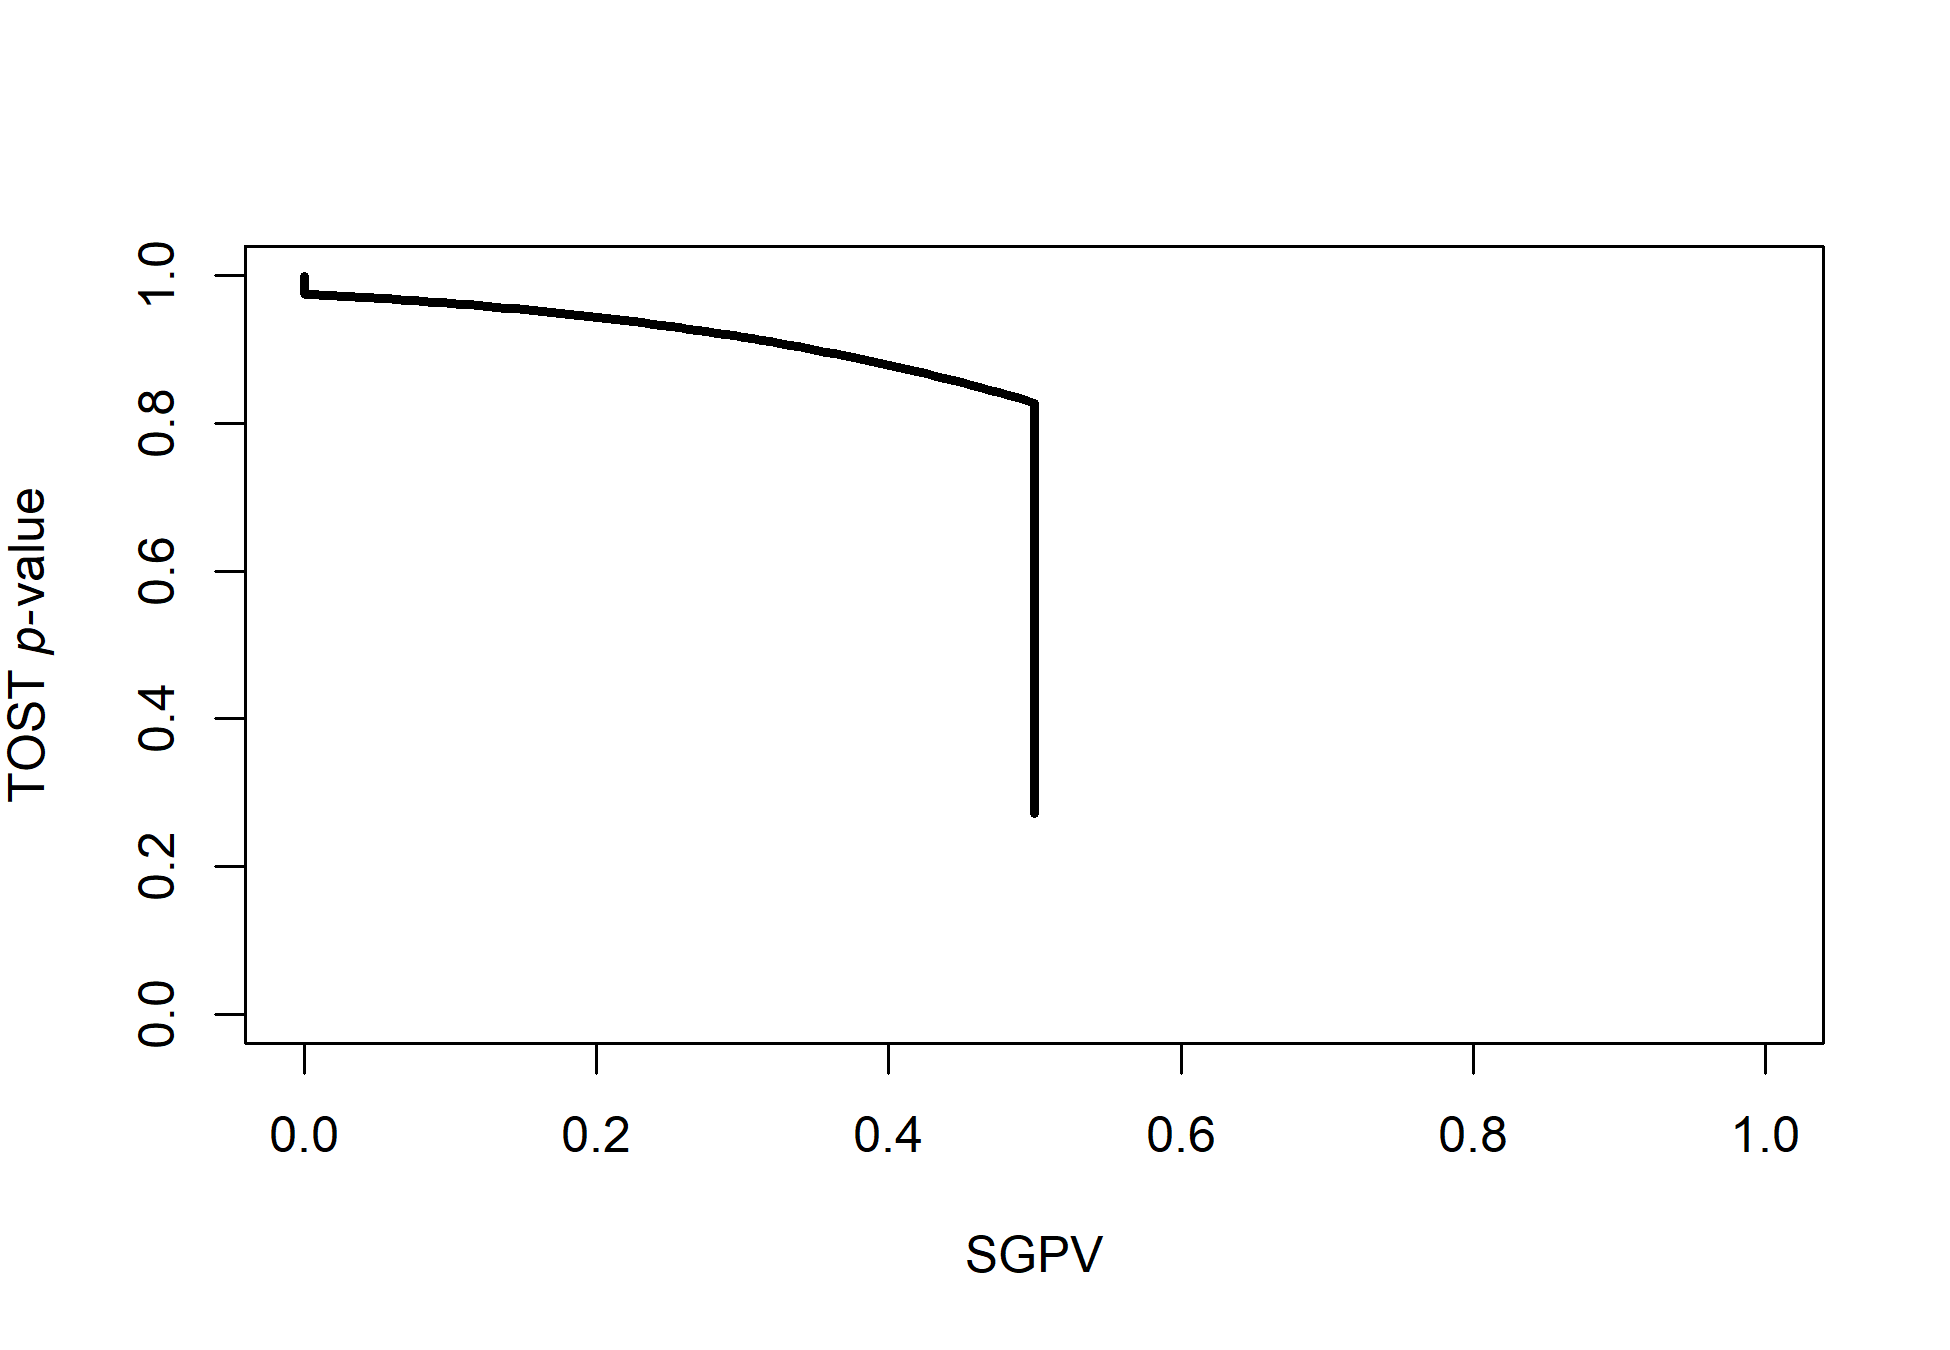
\includegraphics[height=0.94\textheight]{chp5_format-Rmd_bib_files/figure-latex/TOSTSGPV7-1} 

}

\caption{The relationship between $p$-values from the TOST procedure and the SGPV for the same scenario as in Figure \ref{fig:TOSTSGPV6}.}\label{fig:TOSTSGPV7}
\end{figure}

The \emph{p}-value from the TOST procedure still differentiates observed means, while the SGPV does not, when the CI is wider than the equivalence range (so the precision is low) and overlaps with the upper and lower equivalence bound, but the CI is \emph{not} twice as wide as the equivalence range. In the example below, we see that the CI is only 1.79 times as wide as the equivalence bounds, but the CI overlaps with the lower and upper equivalence bounds (Figure \ref{fig:TOSTSGPV8}). This means the SGPV is not set to 0.5, but it is constant across a range of observed means, while the TOST \emph{p}-value is not constant across this range.

\begin{figure}

{\centering 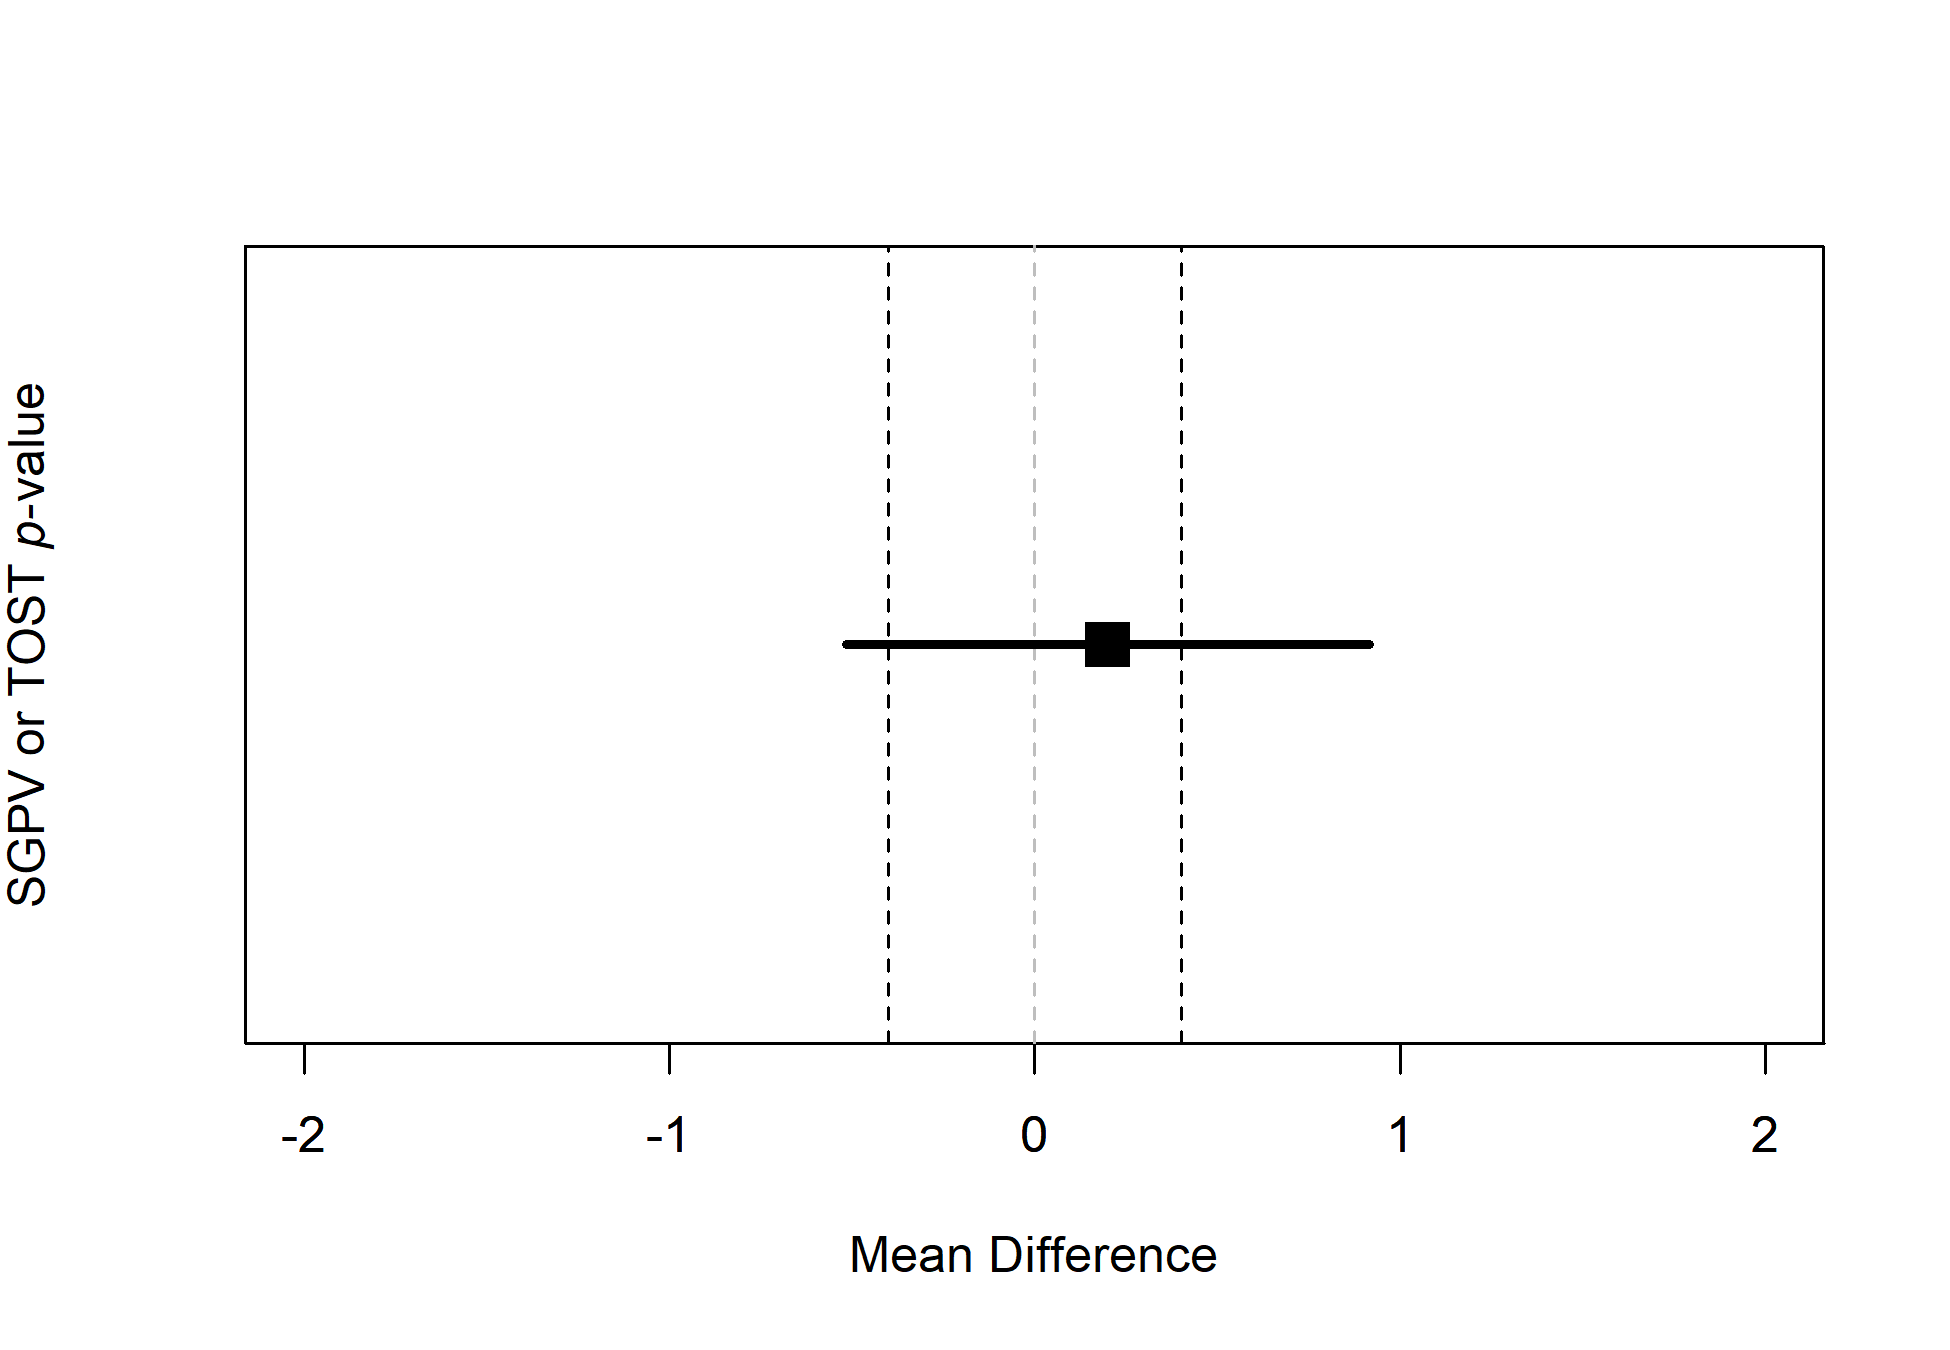
\includegraphics[height=0.94\textheight]{chp5_format-Rmd_bib_files/figure-latex/TOSTSGPV8-1} 

}

\caption{Example of a 95$\%$ CI that overlaps with the lower and upper equivalence bound (indicated by the vertical dotted lines).}\label{fig:TOSTSGPV8}
\end{figure}

If the observed mean would be somewhat closer to 0, or further away from 0, the SGPV remains constant (the CI width does not change, and it completely overlaps with the equivalence range) while the \emph{p}-value for the TOST procedure does vary. We can see this in Figure \ref{fig:TOSTSGPV9} below. The SGPV is not set to 0.5, but is slightly higher than 0.5 across a range of means. How high the SGPV will be for a CI that is not twice as wide as the equivalence range, but overlaps with the lower and upper equivalence bounds, depends on the width of the CI and the equivalence range.

\begin{figure}

{\centering 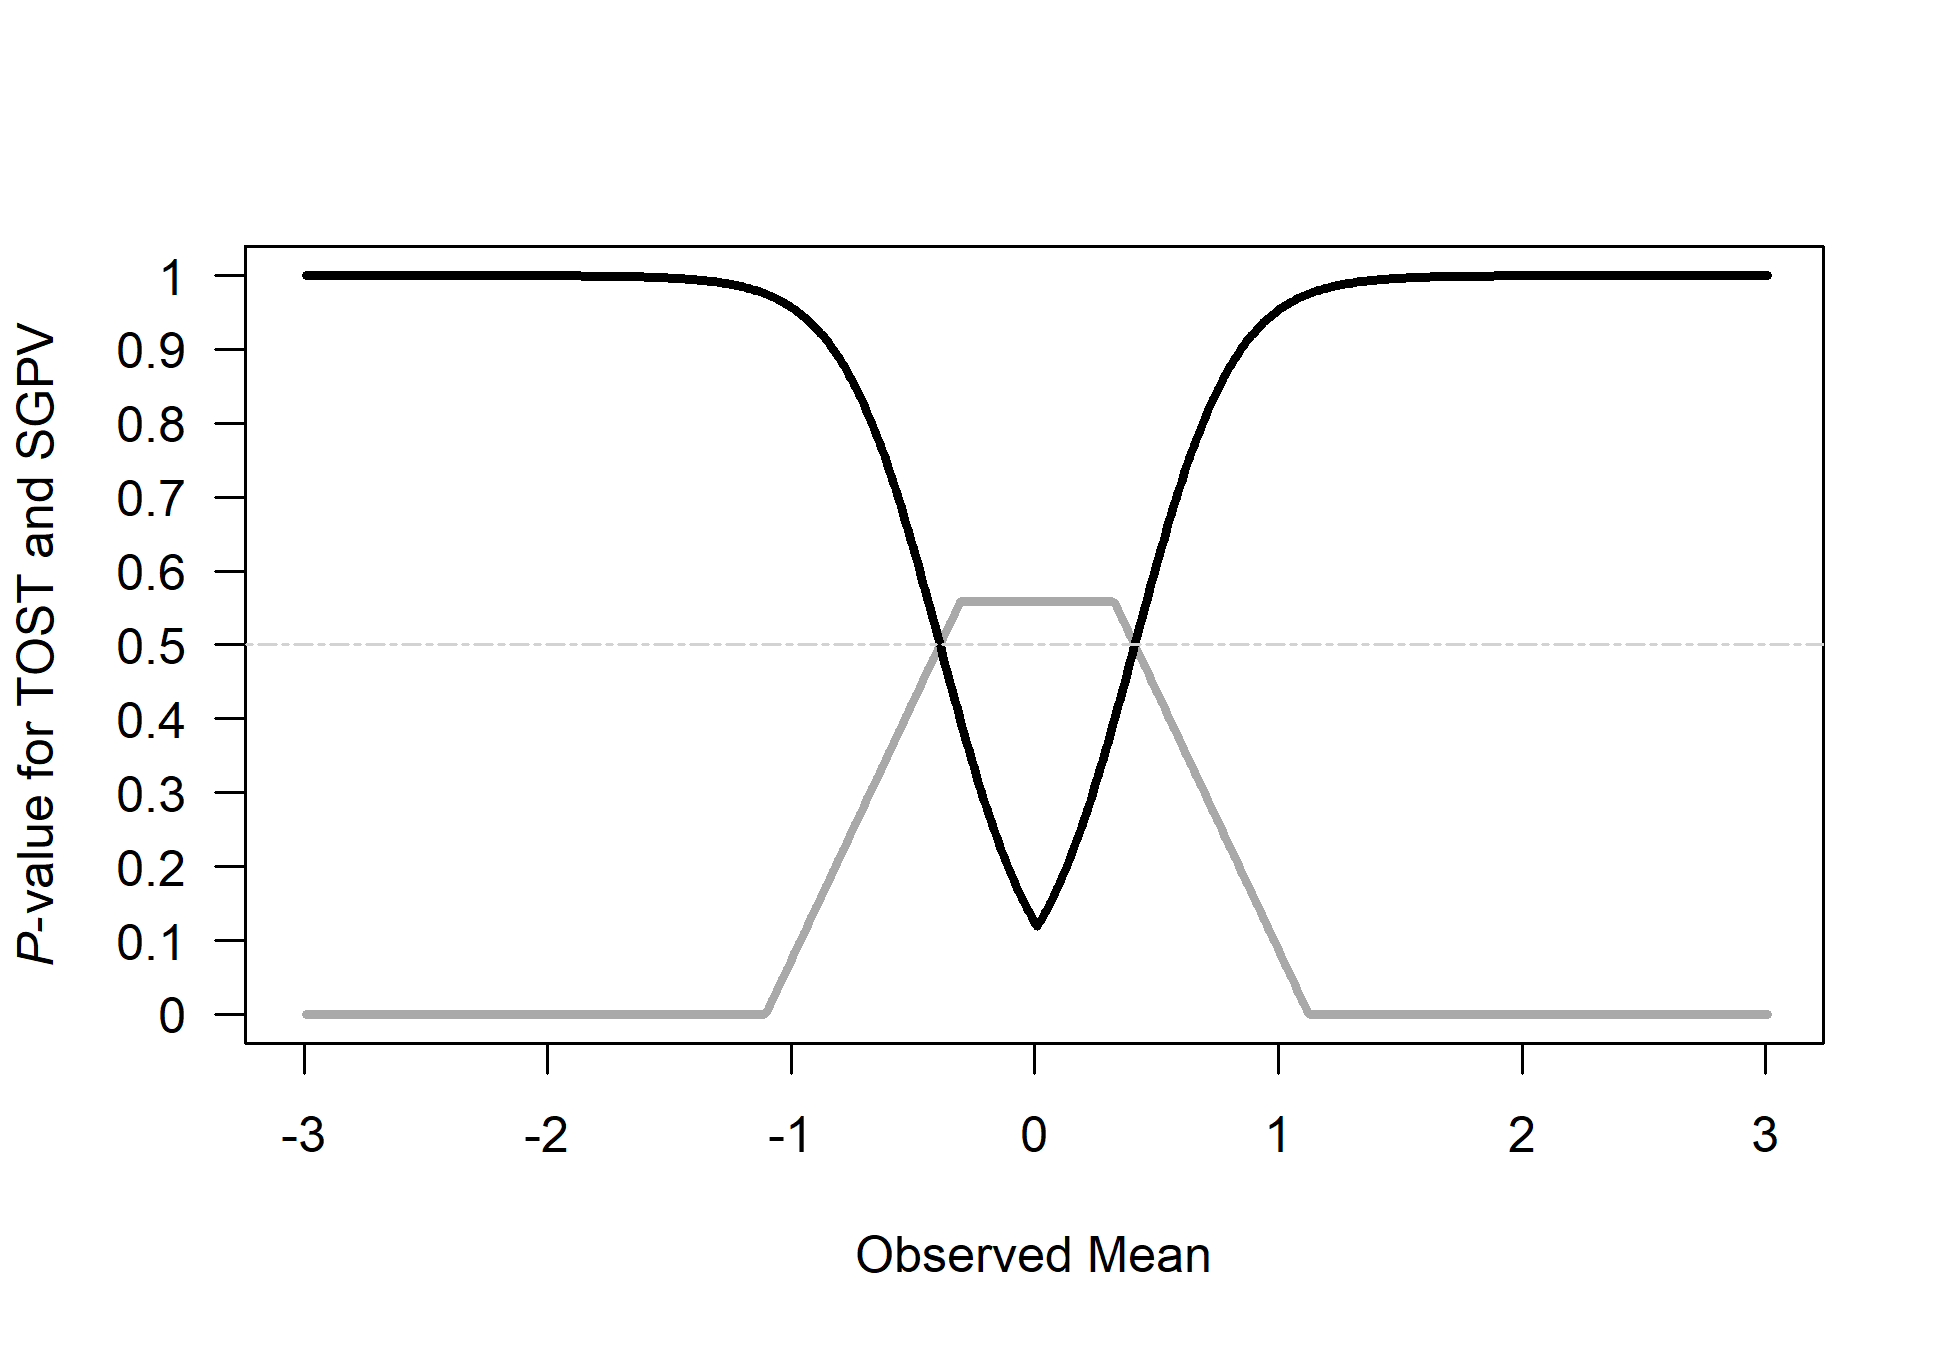
\includegraphics[height=0.94\textheight]{chp5_format-Rmd_bib_files/figure-latex/TOSTSGPV9-1} 

}

\caption{Comparison of $p$-values from TOST (black line) and SGPV (grey line) across a range of observed sample means ($x$-axis). The sample size is small ($n$ = 10), but because the sd is half as big as in Figure \ref{fig:TOSTSGPV7} (1 instead of 2) the CI is less than twice as wide as the equivalence range (set to -0.4 to 0.4). The SGPV is not set to 0.5 (horizontal light grey line) but reaches a maximum slightly above 0.5 across a range of observed means.}\label{fig:TOSTSGPV9}
\end{figure}

If we once more plot the two statistics against each other we see the SGPV is 0.56 for a range of observed means where the \emph{p}-value from the equivalence test still varies, as indicated by the straight section of the line (Figure \ref{fig:TOSTSGPV10}).

\begin{figure}

{\centering 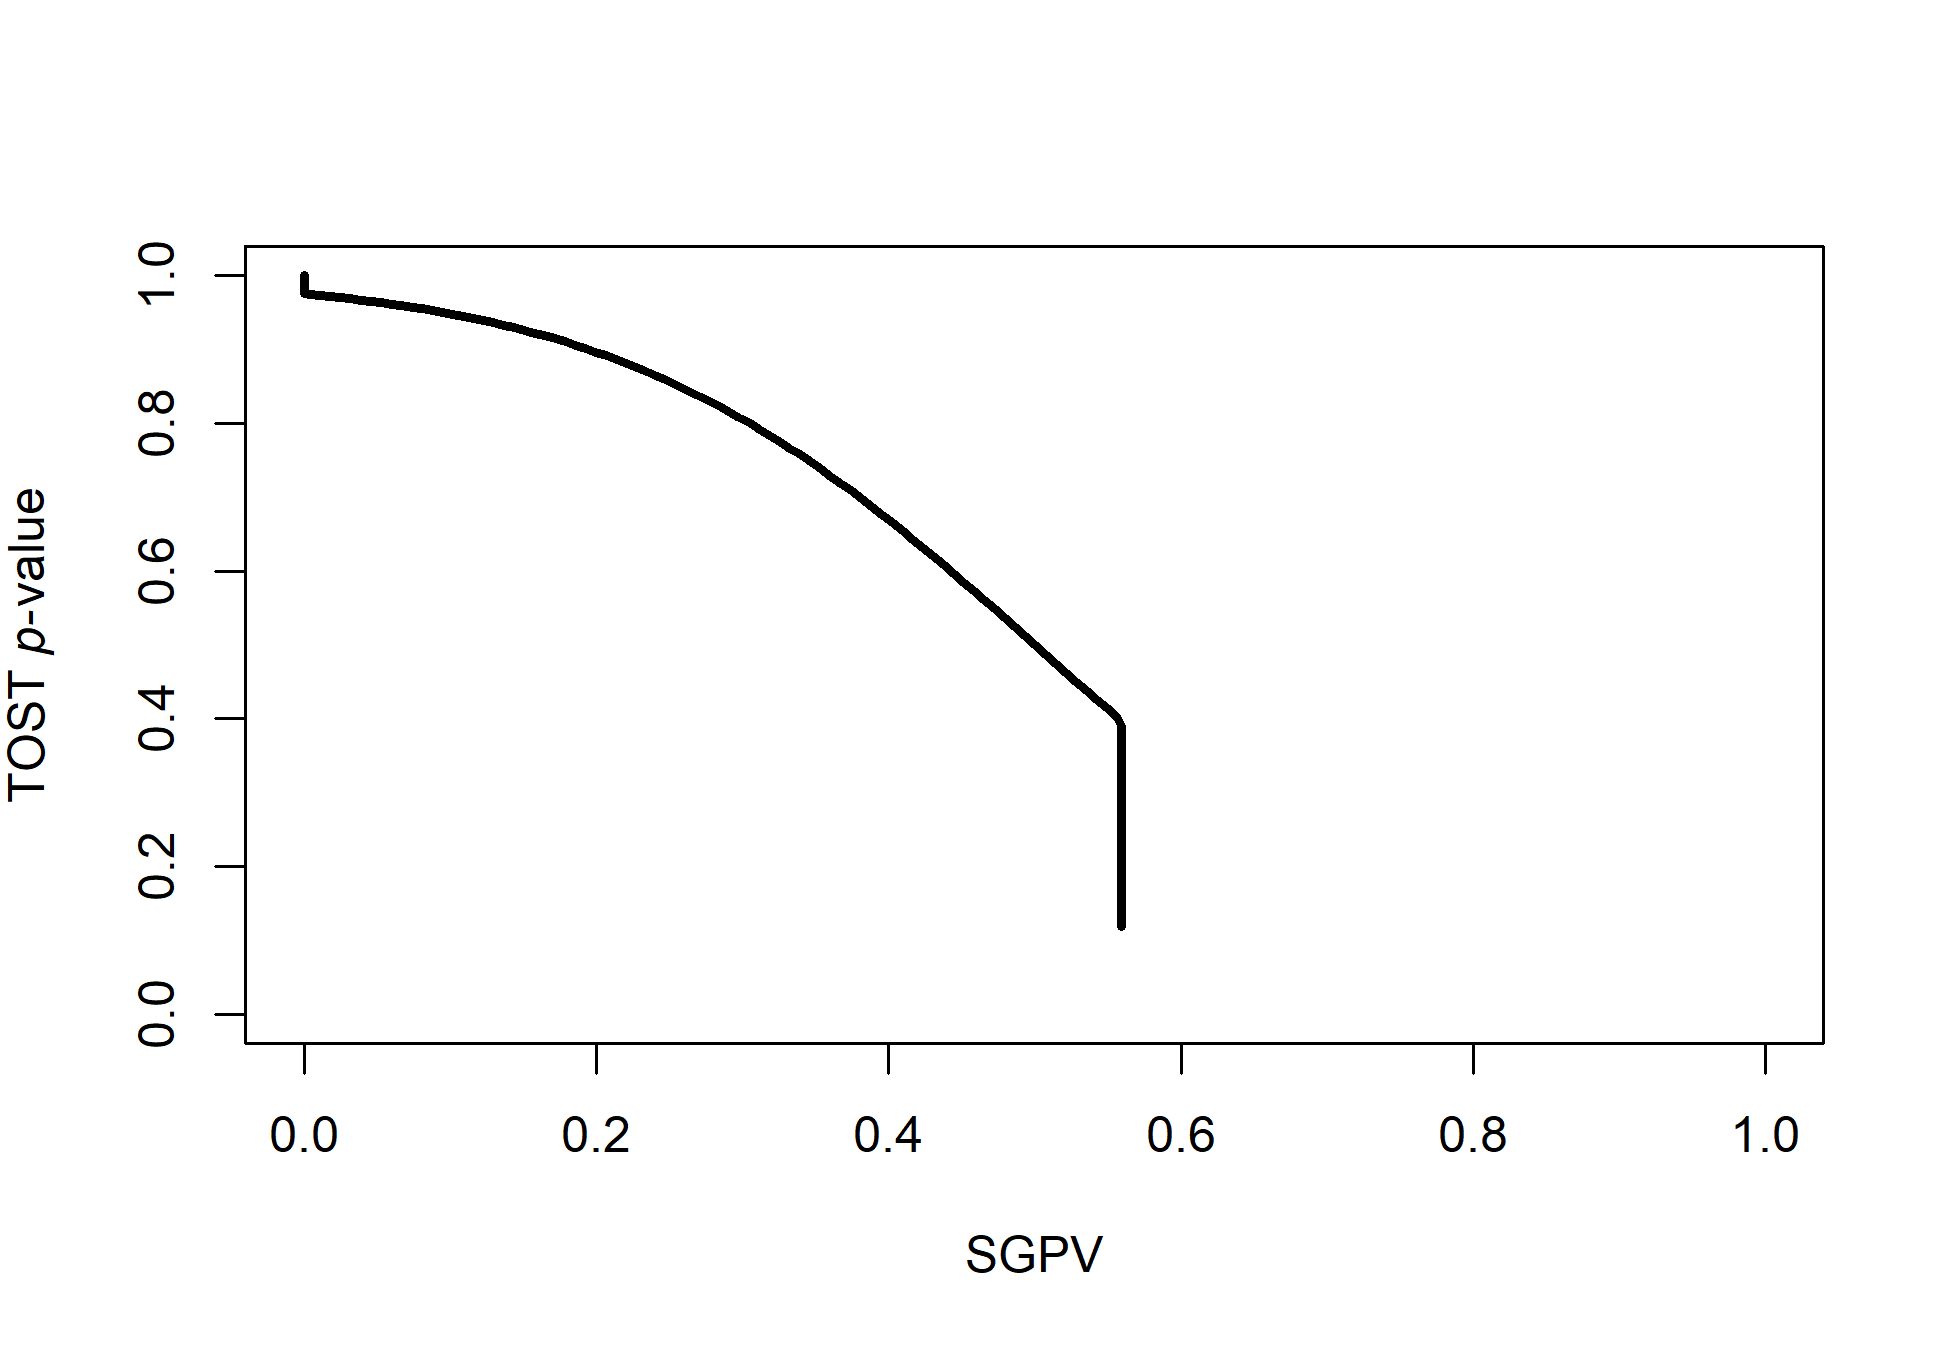
\includegraphics[height=0.94\textheight]{chp5_format-Rmd_bib_files/figure-latex/TOSTSGPV10-1} 

}

\caption{The relationship between $p$-values from the TOST procedure and the SGPV for the same scenario as in Figure \ref{fig:TOSTSGPV9}.}\label{fig:TOSTSGPV10}
\end{figure}

To conclude this section, there are situations where the \emph{p}-value from the TOST procedure continues to differentiate, while the SGPV does not. Therefore, interpreted as a continuous statistic, the SGPV is more limited than the \emph{p}-value from the TOST procedure.

\hypertarget{the-relation-between-equivalence-tests-and-sgpv-for-asymmetrical-confidence-intervals-around-correlations}{%
\paragraph{The relation between equivalence tests and SGPV for asymmetrical confidence intervals around correlations}\label{the-relation-between-equivalence-tests-and-sgpv-for-asymmetrical-confidence-intervals-around-correlations}}

So far we have only looked at the relation between equivalence tests and the SGPV when confidence intervals are symmetric (e.g., for confidence intervals around mean differences). For correlations, which are bound between -1 and 1, confidence intervals are only symmetric for a correlation of exactly 0. The confidence interval for a correlation becomes increasingly asymmetric as the observed correlation nears -1 or 1. For example, with ten observations, an observed correlation of 0 has a symmetric 95\(\%\) confidence interval ranging from -0.63 to 0.63, while and observed correlation of 0.7 has an asymmetric 95\(\%\) confidence interval ranging from 0.13 to 0.92. Note that calculating confidence intervals for a correlation involves a Fisher's z-transformation, which transforms values such that they are approximately normally z-distributed, which allows one to compute symmetric confidence intervals. These confidence intervals are then retransformed into a correlation, where the confidence intervals are asymmetric if the correlation is not exactly zero.

The effect of asymmetric confidence intervals around correlations is most noticeable at smaller sample sizes. In Figure \ref{fig:TOSTSGPV11} we plot the \emph{p}-values from equivalence tests and the SGPV (again plotted as 1-SGPV for ease of comparison) for correlations. The sample size is 30 pairs of observations, and the lower and upper equivalence bounds are set to -0.45 and 0.45, with an alpha of 0.05. As the observed correlation in the sample moves from -.99 to 0 the \emph{p}-value from the equivalence test becomes smaller, as does 1-SGPV. The pattern is quite similar to that in Figure \ref{fig:TOSTSGPV2}. The \emph{p}-value for the TOST procedure and 1-SGPV are still related as discussed above, with TOST \emph{p}-values of 0.975 and 0.025 corresponding to a 1-SGPV of 1 and 0, respectively. There are two important differences, however. First of all, the SGPV is no longer a straight line, but a curve, due to the asymmetry in the 95\(\%\) CI. Second, and most importantly, the \emph{p}-value for the equivalence test and the SGPV do no longer overlap at \emph{p} = 0.5.

\begin{figure}

{\centering 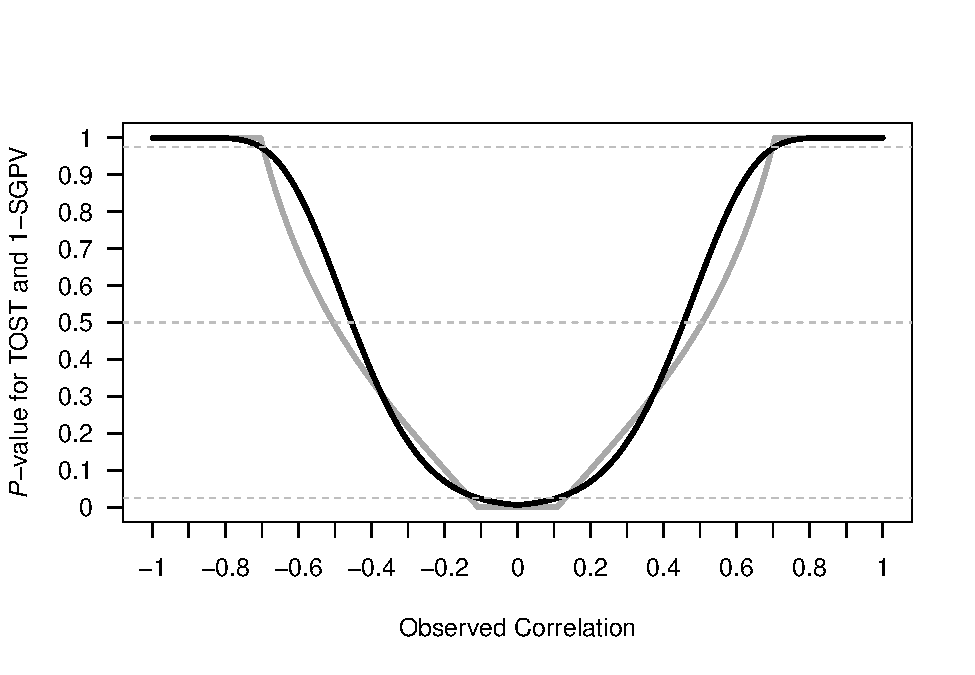
\includegraphics[height=0.94\textheight]{chp5_format-Rmd_bib_files/figure-latex/TOSTSGPV11-1} 

}

\caption{Comparison of $p$-values from TOST (black line) and 1-SGPV (grey curve) across a range of observed sample correlations ($x$-axis) tested against equivalence bounds of $r$ = -0.45 and $r$ = 0.45 with $n$ = 30 and an alpha of 0.05.}\label{fig:TOSTSGPV11}
\end{figure}

The reason that the equivalence test and SGPV no longer overlap is due to asymmetric confidence intervals. If the observed correlation falls exactly on the equivalence bound the \emph{p}-value for the equivalence test is 0.5. In the equivalence test for correlations the \emph{p}-value is computed based on a z-transformation which better controls error rates (\textbf{goertzen\_detecting\_2010?}). This transformation is computed as follows, where \emph{r} is the observed correlation and \(\rho\) is the theoretical correlation under the null :

\[
z = \frac{\frac{\log(\frac{1 + r}{ 1 - r})}{2} - \frac{\log(\frac{1 + \rho}{ 1 - \rho})}{2}}{\sqrt{\frac{1}{n-3}}}
\]

Because the z-distribution is symmetric, the probability of observing the observed or more extreme z-score, assuming the equivalence bound is the true effect size, is 50\(\%\). However, because the \emph{r} distribution is not symmetric, this does not mean that there is always a 50\(\%\) probability of observing a correlation smaller or larger than the true correlation. As can be seen in Figure \ref{fig:TOSTSGPV12}, the proportion of the confidence interval that overlaps with the equivalence range is larger than 50\(\%\) when the observed correlations are \emph{r} = -.45 and \emph{r} = .45, meaning that the two second generation p-values associated with these correlations are larger than 50\(\%\). Because the confidence intervals are asymmetric around the observed effect size of 0.45 (ranging from 0.11 to 0.70) according to (\textbf{blume\_second-generation\_2018?}) 58.11\(\%\) of the data-supported hypotheses are null hypotheses, and therefore 58.11\(\%\) of the data-supported hypotheses are compatible with the null premise.

\begin{figure}

{\centering 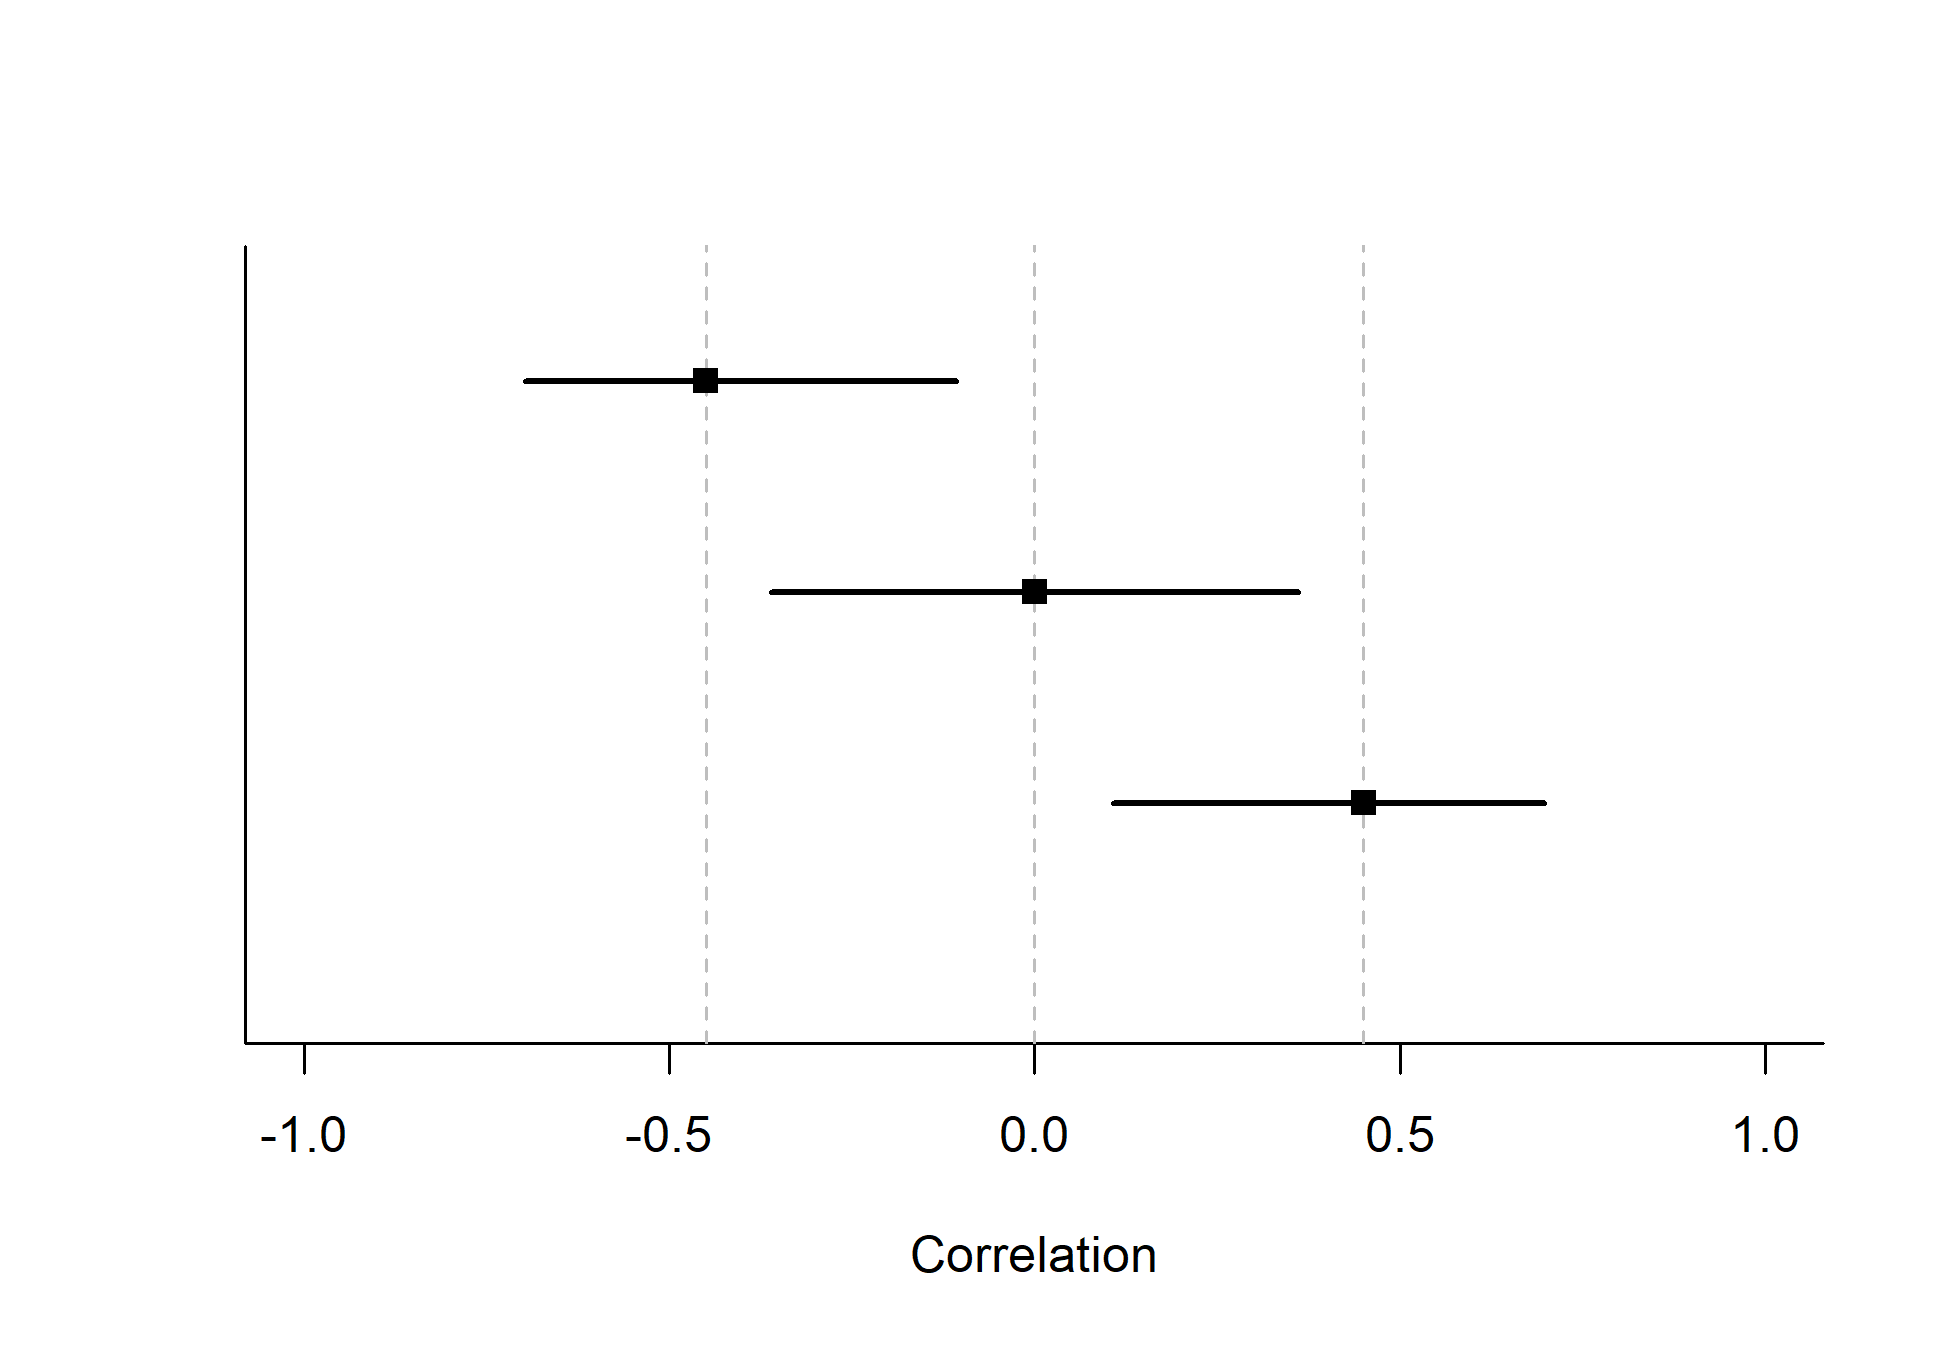
\includegraphics[height=0.94\textheight]{chp5_format-Rmd_bib_files/figure-latex/TOSTSGPV12-1} 

}

\caption{Three 95$\%$ confidence intervals for observed effect sizes of $r$ = -0.45, $r$ = 0, and $r$ = 0.45 for $n$ = 30. Only the confidence interval for $r$ = 0 is symmetric.}\label{fig:TOSTSGPV12}
\end{figure}

The further away from 0, the larger the SGPV when the observed mean falls on the equivalence bound. The SGPV is the proportion of values in a 95\(\%\) confidence interval that overlap with the equivalence range, but not the probability that these values will be observed. In the most extreme case (i.e., a sample size of 4, and equivalence bounds set to \emph{r} = -0.99 and 0.99, with a true correlation of 0.99) 97.60\(\%\) of the confidence interval overlaps with the equivalence range, even though in the long run only 36\(\%\) of the correlations observed in the future will fall in this range.

It should be noted that in larger sample sizes the SGPV is closer to 0.5 whenever the observed correlation falls on the equivalence bound, but this extreme example nevertheless clearly illustrates the difference between question the SGPV answers, and the question a \emph{p}-value answers. The conclusion of this section on asymmetric confidence intervals is that a SGPV of 1 or 0 can still be interpreted as a \emph{p} \textless{} 0.025 or \emph{p} \textgreater{} 0.975 in an equivalence test, since the SGPV and \emph{p}-value for the TOST procedure are always directly related at the values \emph{p} = 0.025 and \emph{p} = 0.975. Although (\textbf{blume\_second-generation\_2018?}) state that ``the degree of overlap conveys how compatible the data are with the null premise'' this definition of what the SGPV provides does not hold for asymmetric confidence intervals. Although a SGPV of 1 or 0 can be directly interpreted, a SGPV between 0 and 1 is not interpretable as `compatibility with the null hypothesis' under the assumption of a bivariate normal distribution, and the generalizability of this statement needs to be examined beyond normal bivariate distributions. Indeed, Blume and colleagues write in the supplemental material that ``The magnitude of an inconclusive second-generation \emph{p}-value can vary slightly when the effect size scale is transformed. However definitive findings, i.e.~a \emph{p}-value of 0 or 1 are \emph{not} affected by the scale changes.''

\hypertarget{what-are-the-relative-strengths-and-weaknesses-of-equivalence-testing-and-the-sgpv}{%
\paragraph{What are the Relative Strengths and Weaknesses of Equivalence Testing and the SGPV?}\label{what-are-the-relative-strengths-and-weaknesses-of-equivalence-testing-and-the-sgpv}}

When introducing a new statistical method, it is important to compare it to existing approaches and specify its relative strengths and weaknesses. Here, we aimed to compare the SGPV against equivalence tests based on the TOST procedure. First of all, even though a SGPV of 1 or 0 has a clear interpretation (we can reject effects outside or inside the equivalence range), intermediate values are not as easy to interpret (especially for effects that have asymmetric confidence intervals). In one sense, they are what they are (the proportion of overlap), but it can be unclear what this number tells us about the data we have collected. This is not too problematic, since the main use of the SGPV (e.g., in all examples provided by Blume and colleagues) seems to be to examine whether the SGPV is 0, 1, or inconclusive. As already mentioned, this interpretation of a SGPV is very similar to the Neyman-Pearson interpretation of an equivalence test and a minimum effect tests (which are complementary). The difference is that where a SGPV of 1 can be interpreted as \emph{p} \textless{} .025, equivalence tests provide exact \emph{p}-values, and they continue to differentiate between for example \emph{p} = 0.024 and \emph{p} = 0.002. Whether this is desirable depends on the perspective that is used. From a Neyman-Pearson perspective on statistical inferences the main conclusion is based on whether or not \(p < \alpha\), and thus an equivalence test and SGPV can be performed by simply checking whether the confidence interval falls within the equivalence range, just as a null-hypothesis test can be performed by checking whether the confidence interval contains zero or not. At the same time, it is recommended to report exact \emph{p}-values (\textbf{association\_publication\_2010?}), and exact \emph{p}-values might provide information of interest to readers about how precisely how surprising the data, or more extreme data, is under the null model. Some researchers might be interested in combining an equivalence test with a null-hypothesis significance test. This allows a researcher to ask whether there is an effect that is statistically different from zero, and whether effect sizes that are considered meaningful can be rejected. Equivalence tests combined with null-hypothesis tests classify results into four possible categories, and for example allow researchers to conclude an effect is significant \emph{and} equivalent (i.e., statistically different from zero, but also too small to be considered meaningful; see Lakens et al., 2018).

An important issue when calculating the SGPV is its reliance on the `small sample correction,' where the SGPV is set to 0.5 whenever the ratio of the confidence interval width to the equivalence range exceeds 2:1 and the CI overlaps with the upper and lower bounds. This exception to the normal calculation of the SGPV is introduced to prevent misleading values. Without this correction it is possible that a confidence interval is extremely wide, and an equivalence range is extremely narrow, which without the correction would lead to a very low value for the SGPV. (\textbf{blume\_second-generation\_2018?}) suggest that under such a scenario `the data favor alternative hypotheses,' even when a better interpretation would be that there is not enough data to accurately estimate the true effect compared to the width of the equivalence range. Although it is necessary to set the SGPV to 0.5 whenever the ratio of the confidence interval width to the equivalence range exceeds 2:1, it leads to a range of situations where the SGPV is set to 0.5, while the \emph{p}-value from the TOST procedure continues to differentiate (see for example Figure \ref{fig:TOSTSGPV6}). An important benefit of equivalence tests is that it does not need such a correction to prevent misleading results.

\begin{figure}

{\centering 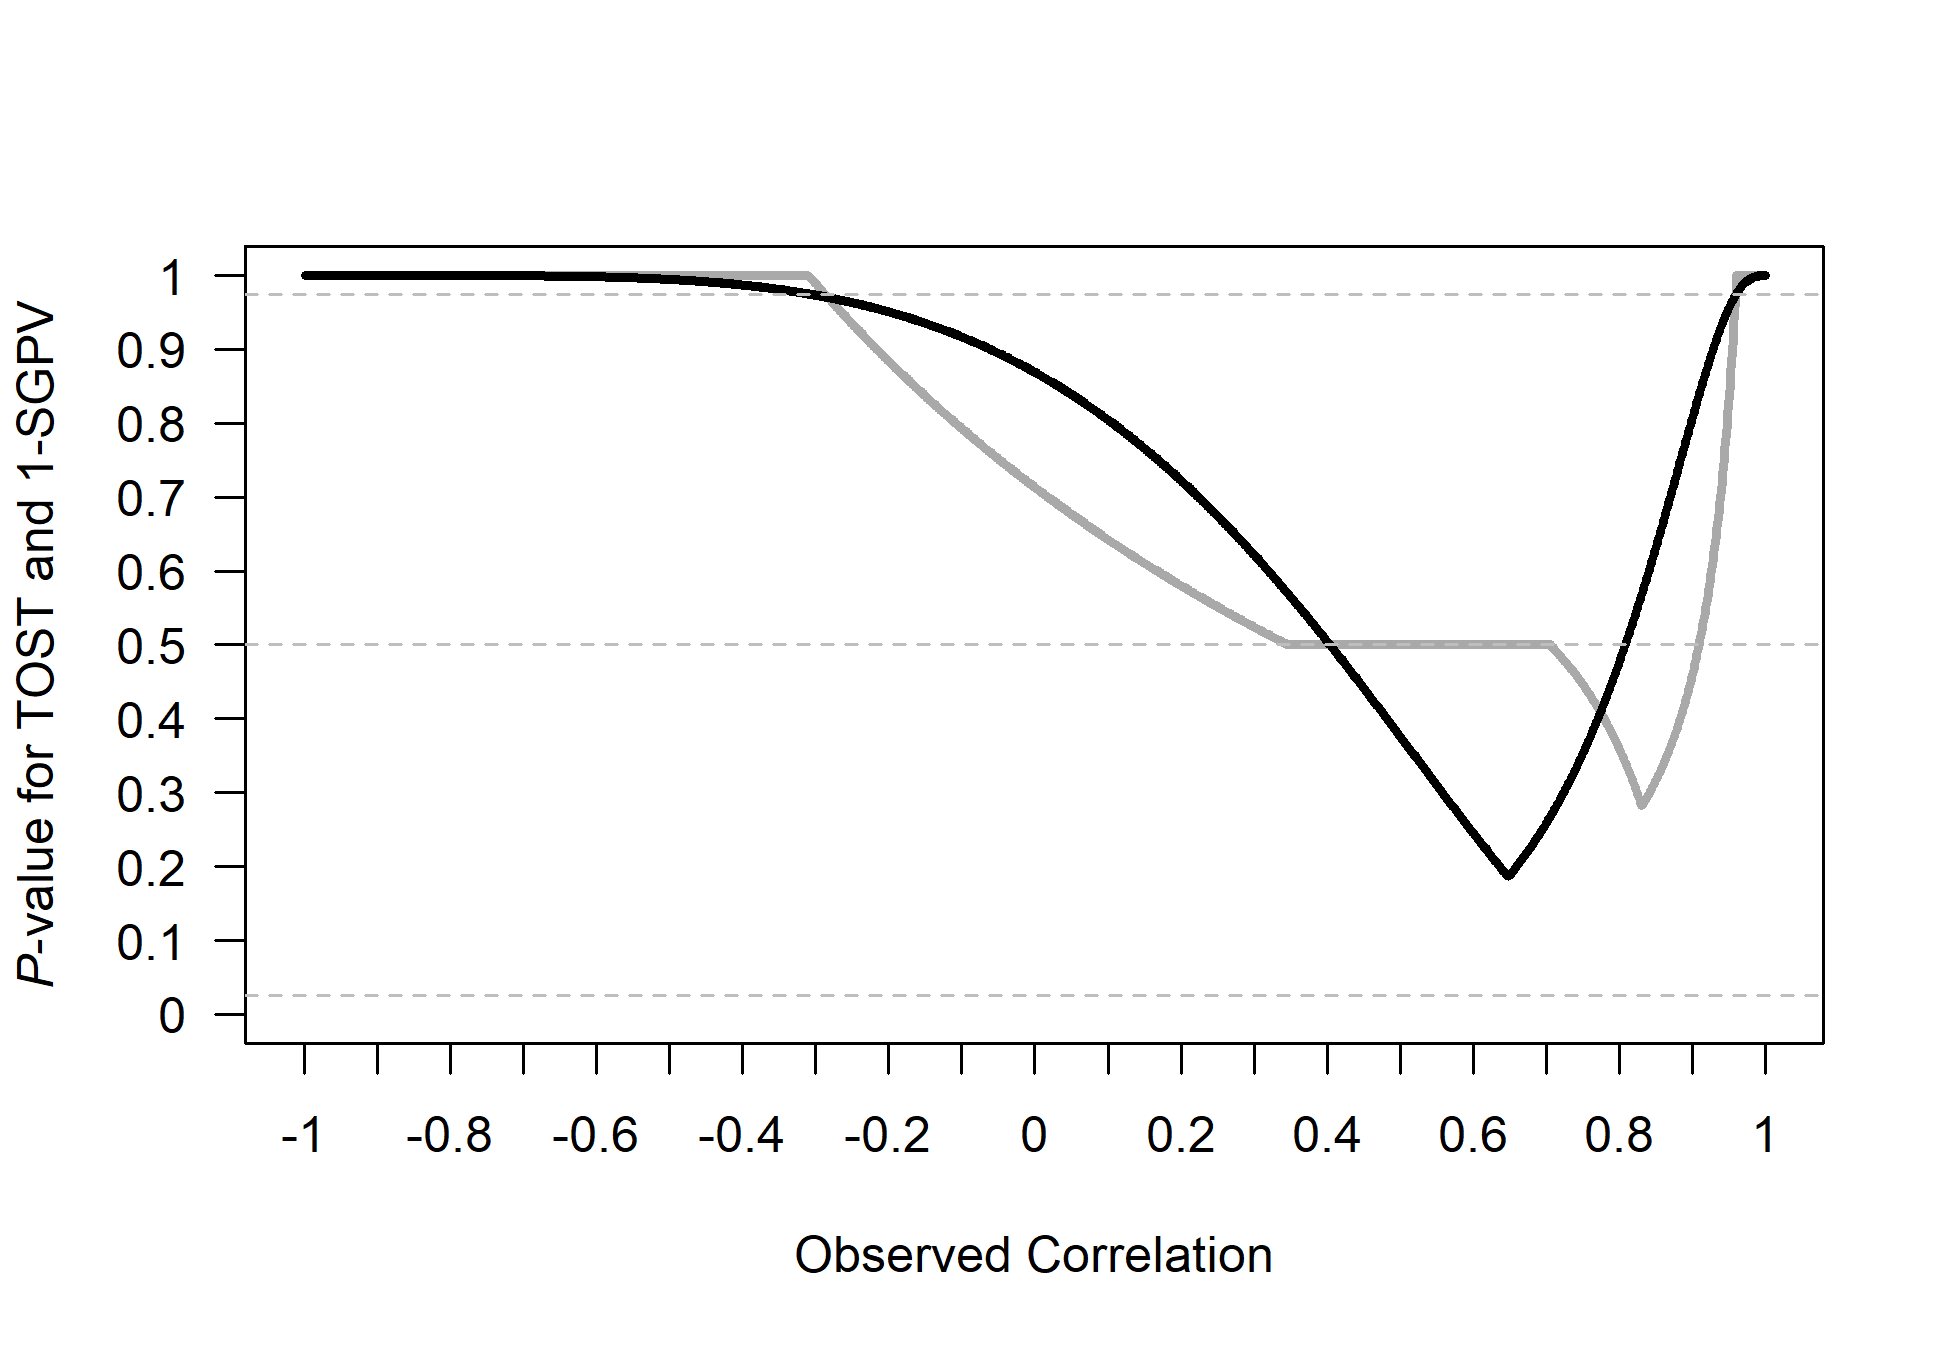
\includegraphics[height=0.94\textheight]{chp5_format-Rmd_bib_files/figure-latex/TOSTSGPV13-1} 

}

\caption{Comparison of $p$-values from TOST (black line) and 1-SGPV (grey curve) across a range of observed sample correlations ($x$-axis) tested against equivalence bounds of $r$ = 0.4 and $r$ = 0.8 with $n$ = 10 and an alpha of 0.05.}\label{fig:TOSTSGPV13}
\end{figure}

As a more extreme example of the peculiar behavior of the `small sample correction' as currently implemented in the calculation of the SGPV, see Figure \ref{fig:TOSTSGPV13}. In this figure observed correlations (from a sample size of 10) from -.99 to .99 are tested against an equivalence range from r = 0.4 to r = 0.8. We can see the SGPV has a peculiar shape because it is set to 0.5 for certain observed correlations, even though there is no risk of a `misleading' SGPV in this range. This example suggests that the current implementation of the `small sample correction' could be improved. If, on the other hand, the SGPV is mainly meant to be interpreted when it is 0 or 1, it might be preferable to simply never apply the `small sample correction.'

(\textbf{blume\_second-generation\_2018?}) claim that when using the SGPV ``Adjustments for multiple comparisons are obviated'' (p.~15). However, this is not correct. Given the direct relationship between TOST and SGPV highlighted in this manuscript (where a TOST \emph{p} = 0.025 equals SGPV = 1, as long as the SGPV is calculated based on confidence intervals, and assuming data are sampled from a continuous bivariate normal distribution), not correcting for multiple comparisons will inflate the probability of concluding the absence of a meaningful effect based on the SGPV in exactly the same way as it will for equivalence tests. Whenever statistical tests are interpreted as support for a hypothesis (e.g., SPGV = 0 or SGPV = 1), it is possible to do so erroneously, and if researchers want to control error rates, they need to correct for multiple comparisons.

\hypertarget{conclusion}{%
\subsubsection{Conclusion}\label{conclusion}}

We believe that our explanation of the similarities between the TOST procedure and the SGPV provides context to interpret the contribution of second generation \emph{p}-values to the statistical toolbox. The novelty of the SGPV can be limited when confidence intervals are asymmetrical or wider than the equivalence range. There are strong similarities with \emph{p}-values from the TOST procedure, and in all situations where the statistics yield different results, the behavior of the \emph{p}-value from the TOST procedure is more consistent. We hope this overview of the relationship between the SGPV and equivalence tests will help researchers to make an informed decision about which statistical approach provides the best answer to their question. Our comparisons show that when proposing alternatives to null-hypothesis tests, it is important to compare new proposals to already existing procedures. We believe equivalence tests achieve the goals of the second generation \emph{p}-value while allowing users to easily control error rates, and while yielding more consistent statistical outcomes.


\end{document}
